\documentclass[12pt,a4paper]{article}

\usepackage[utf8]{inputenc}
\usepackage[french]{babel}
\usepackage[T1]{fontenc}

\usepackage{amsmath}
\usepackage{amsfonts}
\usepackage{amssymb}

% Preparation des infos generales
\newcommand{\TitreMatiere}{Python}
\newcommand{\DateExo}{12 septembre 2023}
\newcommand{\AnneeScolaire}{2023-2024}
\newcommand{\Organisation}{EPITA}
\newcommand{\TypeExo}{Projet}
\newcommand{\TitreExercice}{Statistiques}
\newcommand{\NomAuteurA}{Fabrice BOISSIER}
\newcommand{\MailAuteurA}{fabrice.boissier@epita.fr}
\newcommand{\NomAuteurB}{Lisa MONPIERRE}
\newcommand{\MailAuteurB}{lisa.monpierre@epita.fr}
\newcommand{\VersionExo}{Version 3}
\newcommand{\LoginEtudiant}{2023-2024} % Watermark de protection

%\newcommand{\RenduTarball}{nom1-nom2-TP1.tar.bz2}
%\newcommand{\RenduDir}{nom1-nom2-TP1}
\newcommand{\RenduTarball}{login-Python-Stats.tar.bz2}
\newcommand{\RenduDir}{login-Python-Stats}


% Ajout de mes classes & definitions
\usepackage{MetalExo} % Appelle un .sty


% Redefinition headers
\lhead{\TitreExercice}		%Gauche Haut
\chead{\TypeExo}			%Centre Haut
\rhead{\thepage}			%Droite Haut
\lfoot{}					%Gauche Bas
\cfoot{\TitreMatiere}		%Centre Bas
\rfoot{}					%Droite Bas


\definecolor{mygreen}{rgb}{0,0.6,0}		% RGB model
\definecolor{mygray}{rgb}{0.5,0.5,0.5}
\definecolor{mymauve}{rgb}{0.58,0,0.82}


\usepackage{array}
\newcolumntype{P}[1]{>{\raggedright\arraybackslash }m{#1}}

\newcolumntype{L}[1]{>{\raggedright\arraybackslash }b{#1}}
\newcolumntype{C}[1]{>{\centering\arraybackslash }b{#1}}
\newcolumntype{R}[1]{>{\raggedleft\arraybackslash }b{#1}}

\newcolumntype{G}[1]{>{\raggedright\let\newline\\\arraybackslash\hspace{0pt}}m{#1}} % another L
\newcolumntype{M}[1]{>{\centering\let\newline\\\arraybackslash\hspace{0pt}}m{#1}}   % another C
\newcolumntype{D}[1]{>{\raggedleft\let\newline\\\arraybackslash\hspace{0pt}}m{#1}}  % another R

\begin{document}

%% Titre
\maketitle

%\newpage

%% Copyright
\pagenumbering{Roman}

%% Copyright

{\Large \textbf{Copyright}}

\vspace{30px}

Ce document est destiné à l'usage interne de Paris 1 - Panthéon Sorbonne.\\

Copyright \space \copyright \space Fabrice BOISSIER - 2019\\

\bigskip

\begin{center}
	\fcolorbox{black}{white}{\makebox[14cm]{
	\begin{minipage}[l]{12cm}
		\vspace*{10px}
		\textbf{Ce document est soumis à conditions :}
		\medskip

		Il est interdit de partager ce document avec d'autres personnes.
		\smallskip

		Vérifiez que vous disposez de la dernière révision de ce document.
	\vspace*{10px}
	\end{minipage}
	}}
\end{center}


\newpage

%% Table des matieres
\tableofcontents

\newpage

%% Consignes generales
\section{Consignes Générales}

\bigskip

%% Consignes generales
\noindent \textit{Les informations suivantes sont très importantes :}

\bigskip

\noindent \textit{Le non-respect d'une des consignes suivantes entraînera des sanctions pouvant aller jusqu'à la multiplication de la note finale par 0.}

\bigskip

\noindent \textit{Ces consignes sont claires, non-ambiguës, et ont un objectif précis. En outre, elles ne sont pas négociables.}

\bigskip

\noindent N'hésitez pas à demander si vous ne comprenez pas une des règles.

\bigskip

\newcounter{My_Counter}

\ConsigneGenerale{My_Counter}{Vous devez lire le sujet.}
\ConsigneGenerale{My_Counter}{Vous devez respecter les consignes.}
\ConsigneGenerale{My_Counter}{Vous devez rendre le travail dans les délais prévus.}

\medskip

\ConsigneGenerale{My_Counter}{Le travail doit être rendu dans le format décrit à la section \hyperref[sec:FormatDeRendu]{Format de Rendu}.}

\ConsigneGenerale{My_Counter}{Le travail rendu ne doit pas contenir de fichiers binaires, temporaires, ou d'erreurs (\texttt{\textbf{*\textasciitilde}}, \texttt{\textbf{*.o}}, \texttt{\textbf{*.a}}, \texttt{\textbf{*.so}}, \texttt{\textbf{*\#*}}, \texttt{\textbf{*core}}, \texttt{\textbf{*.log}}, \texttt{\textbf{*.exe}}, binaires, ...).}

\ConsigneGenerale{My_Counter}{Dans l'ensemble de ce document, la casse (caractères majuscules et minuscules) est très importante. Vous devez strictement respecter les majuscules et minuscules imposées dans les messages et noms de fichiers du sujet.}

%\ConsigneGenerale{My_Counter}{Dans l'ensemble de ce document, \LoginX \space correspond à votre login.}
\ConsigneGenerale{My_Counter}{Dans l'ensemble de ce document, \TTBF{nom1-nom2} \space correspond à la combinaison des deux noms de votre binôme (par exemple pour Fabrice BOISSIER et Mark ANGOUSTURES, cela donnera \TTBF{boissier-angoustures}).}

\ConsigneGenerale{My_Counter}{Dans l'ensemble de ce document, le caractère \TTBF{\textvisiblespace } correspond à une espace (s'il vous est demandé d'afficher \TTBF{\textvisiblespace \textvisiblespace \textvisiblespace }, vous devez afficher trois espaces consécutives).}

\ConsigneGenerale{My_Counter}{Tout retard, même d'une seconde, entraîne la note non négociable de 0.}

\ConsigneGenerale{My_Counter}{La triche (échange de code, copie de code ou de texte, ...) entraîne \textbf{au mieux} la note non négociable de 0.}

\ConsigneGenerale{My_Counter}{En cas de problème avec le projet, vous devez contacter le plus tôt possible les responsables du sujet aux adresses mail indiquées.}

\bigskip

\noindent \textbf{Conseil :} N'attendez pas la dernière minute pour commencer à travailler sur le sujet.


\newpage

%% Format de Rendu
\section{Format de Rendu}
\label{sec:FormatDeRendu}

\vspace*{1cm}

%% Format de Rendu

%\ResponsablesProjet{Metal Man/metalman@example.org, Damdoshi/damdoshi@example.org, Tayst/tayst@tayst.org}
%\begin{tabular}{p{7cm} p{10cm}}
\begin{tabular}{p{7cm} p{8.5cm}}
	%\ResponsablesProjetRow{Fabrice BOISSIER/fabrice.boissier@univ-paris1.fr, Ali JAFFAL/ali.jaffal@univ-paris1.fr}
	\ResponsablesProjetRow{Fabrice BOISSIER/fabrice.boissier@epita.fr}
	& \\
%	\RenduSpecsGenerales{[PHP][DM]}{2}{Envoi par mail}{\RenduDir}{\RenduTarball}{10/02/2020 23h42}{2 semaines}
%	\RenduSpecsGenerales{[CAV][TP1]}{1}{Pas de rendu}{\RenduDir}{\RenduTarball}{Pas de rendu}{Pas de rendu}
	\RenduSpecsGenerales{[C][STR]}{1}{Devoir/Assignment sur Teams}{\RenduDir}{\RenduTarball}{18/12/2022 23h42}{2 semaines}
	& \\
%	\RenduSpecsTechniques{WAMP ou MAMP}{PHP}{Apache/PHP}{ }
%	\RenduSpecsTechniques{Linux - Ubuntu (x86\_64)}{C}{/usr/bin/gcc}{-W -Wall -Werror -std=c99 -pedantic}
	\RenduSpecsTechniques{Linux}{C}{gcc}{-W -Wall -Werror -std=c99 -pedantic}
%	& \\
%	Fonctions autorisées : & malloc(3), free(3), printf(3)
\end{tabular}


\vspace*{1cm}


\noindent Les fichiers suivants sont requis :

\medskip

\begin{tabular}{l p{12cm}}
\texttt{AUTHORS} & contient le(s) nom(s) et prénom(s) de(s) auteur(s).\\
%\texttt{Makefile} & le Makefile principal.\\
\texttt{README} & contient la description du projet et des exercices, ainsi que la fa\c con d'utiliser le projet.\\
%\texttt{configure} & le script shell de configuration pour l'environnement de compilation.\\
\end{tabular}


\vspace*{1cm}


%\noindent Un fichier \TTBF{Makefile} doit être présent à la racine du dossier, et doit obligatoirement proposer ces règles :

\medskip

%\begin{tabular}{l p{13cm}}
%\texttt{all} & \textit{[Première règle]} lance la règle \texttt{libmyqueue}.\\
%\texttt{clean} & supprime tous les fichiers temporaires et ceux créés par le compilateur.\\
%\texttt{dist} & crée une archive propre, valide, et répondant aux exigences de rendu.\\
%\texttt{distclean} & lance la règle \texttt{clean}, puis supprime les binaires et bibliothèques.\\
%\texttt{check} & lance le(s) script(s) de test.\\
%\texttt{libmyqueue} & lance les règles \texttt{shared} et \texttt{static} \\
%\texttt{shared} & compile l'ensemble du projet avec les options de compilations exigées et génère une bibliothèque dynamique.\\
%\texttt{static} & compile l'ensemble du projet avec les options de compilations exigées et génère une bibliothèque statique.\\
%\end{tabular}


%\vspace*{1cm}
%\newpage

\noindent Votre code sera testé automatiquement, vous devez donc scrupuleusement respecter les spécifications pour pouvoir obtenir des points en validant les exercices.
%
Votre code sera testé en l'intégrant à une série de tests automatisés qui seront fournis un peu plus tard.
N'attendez SURTOUT PAS que ces tests soient envoyés pour commencer à produire vos fonctions et vos propres tests.
%
%Votre code sera testé en générant un exécutable ou des bibliothèques avec les commandes suivantes :

%\medskip
%
%\begin{tabular}{l}
%\texttt{./configure}\\
%\texttt{make}\\
%\end{tabular}
%
%\bigskip
%
%\noindent Suite à cette étape de génération, les exécutables ou bibliothèques doivent être placés à ces endroits :
%
%\medskip
%
%\begin{tabular}{l}
%\TTBF{\RenduDir/libmyqueue.a}\\
%\TTBF{\RenduDir/libmyqueue.so}\\
%\end{tabular}

\bigskip

\noindent L'arborescence attendue pour le projet est la suivante :

\medskip

\begin{tabular}{l}
\TTBF{\RenduDir/}\\
\TTBF{\RenduDir/AUTHORS}\\
\TTBF{\RenduDir/README}\\
%\TTBF{\RenduDir/Makefile}\\
%\TTBF{\RenduDir/configure}\\
%\TTBF{\RenduDir/check/}\\
%\TTBF{\RenduDir/check/check.sh}\\
\TTBF{\RenduDir/src/}\\
\TTBF{\RenduDir/src/StrBasics.c}\\
\TTBF{\RenduDir/src/StrBasics.h}\\
\TTBF{\RenduDir/src/StrPart1.c}\\
\TTBF{\RenduDir/src/StrPart1.h}\\
\TTBF{\RenduDir/src/StrPart2.c}\\
\TTBF{\RenduDir/src/StrPart2.h}\\
%\TTBF{\RenduDir/src/StrBonus.c}\\
%\TTBF{\RenduDir/src/StrBonus.h}\\
\end{tabular}


\vspace*{1cm}


%\noindent \textit{Vous ne serez jamais pénalisés pour la présence de makefiles ou de fichiers sources (code et/ou headers) dans les différents dossiers du projet tant que leur existence peut être justifiée (des makefiles vides ou jamais utilisés sont pénalisés).}

%\noindent \textit{Vous ne serez jamais pénalisés pour la présence de fichiers de différentes natures dans le dossier \texttt{check} tant que leur existence peut être justifiée (des fichiers de test jamais utilisés sont pénalisés).}


%%%%%%%%%%%%%%%%%%%%%%%%%%%%
%% AIDE MEMOIRE AU CAS OU %%
%%%%%%%%%%%%%%%%%%%%%%%%%%%%
\newpage

\section{Aide Mémoire}
\label{sec:AideMemoire}

\vspace*{1cm}

%%%%%%%%%%%%%%%%%%%%%%%%%%%%
%% AIDE MEMOIRE AU CAS OU %%
%%%%%%%%%%%%%%%%%%%%%%%%%%%%
%\newpage

%{\Large \textbf{Aide Mémoire}}

%\vspace{30px}

%\noindent Le travail doit être rendu au format \textbf{\textit{.zip}}, c'est-à-dire une archive \textbf{zip} compressée avec un outil adapté (les logiciels \textit{7zip} ou \textit{Keka} sont gratuits et adaptés).
\noindent Le travail doit être rendu au format \textbf{\textit{.tar.bz2}}, c'est-à-dire une archive \textbf{bz2} compressée avec un outil adapté (voir \TTBF{man 1 tar} et \TTBF{man 1 bz2}).

%\noindent Tout autre format d'archive (rar, 7zip, gz, gzip, bzip, ...) ne sera pas pris en compte, et votre travail ne sera pas corrigé (entraînant la note de 0).
\noindent Tout autre format d'archive (zip, rar, 7zip, gz, gzip, ...) ne sera pas pris en compte, et votre travail ne sera pas corrigé (entraînant la note de 0).

\bigskip

\noindent Pour générer une archive \textit{tar} en y mettant les dossiers \textit{folder1} et \textit{folder2}, vous devez taper :

\TTBF{tar cvf MyTarball.tar folder1 folder2}


\bigskip


\noindent Pour générer une archive \textit{tar} et la compresser avec GZip, vous devez taper :

\TTBF{tar cvzf MyTarball.tar.gz folder1 folder2}


\bigskip


\noindent Pour générer une archive \textit{tar} et la compresser avec BZip2, vous devez taper :

\TTBF{tar cvjf MyTarball.tar.bz2 folder1 folder2}


\bigskip


\noindent Pour lister le contenu d'une archive \textit{tar}, vous devez taper :

\TTBF{tar tf MyTarball.tar.bz2}


\bigskip


\noindent Pour extraire le contenu d'une archive \textit{tar}, vous devez taper :

\TTBF{tar xvf MyTarball.tar.bz2}


\vspace*{1cm}

%\noindent Dans ce sujet précis, vous ferez du code en C et des appels à des scripts shell qui afficheront les résultats dans le terminal (donc des flux de sortie qui pourront être redirigés vers un fichier texte).

%\noindent Dans ce sujet précis, vous ferez du code en script shell, qui affichera les résultats dans le terminal (donc des flux de sortie qui pourront être redirigés vers un fichier texte).

%\noindent Dans ce sujet précis, vous ferez du code en PHP, qui affichera les résultats dans une page HTML. Les valeurs seront affichées dans une \textit{textarea} dont le texte est généré par des outils multiplateformes supportant les retours à la ligne UNIX (\textbf{\textbackslash n}). Il ne faut donc pas inclure de balise \TTBF{"<br />"} pour retourner à la ligne, mais un \TTBF{"\textbackslash n"}.

\noindent Dans ce sujet précis, vous ferez du code en Python, qui affichera les résultats dans le terminal (donc des flux de sortie qui pourront être redirigés vers un fichier texte).

%\vspace*{1cm}

%\noindent Pour réaliser le travail demandé, nous vous fournirons pour chaque exercice au moins 2 fichiers : \TTBF{exoN\_res.php} (le fichier qui sera appelé pour voir le résultat de votre travail), et \TTBF{exoN\_fun.php} (le fichier contenant la fonction que vous devez coder dans chaque exercice).
%Optionnellement, un fichier \TTBF{exoN\_data.php} peut être fourni pour indiquer le format de données en entrée.
%Le \TTBF{N} correspond au numéro de l'exercice.

%\medskip

%\noindent Dans tous les cas, vous ne devez rendre que le fichier \TTBF{exoN\_fun.php} avec au moins la fonction demandée remplie (qui peut faire appel à d'autres fonctions que vous définirez dans le \textbf{même} fichier). Les autres fichiers seront générés par nos soins pour tester vos fonctions.

%\vspace*{1cm}

%\noindent Vous ne devez \textbf{PAS} utiliser la fonction \TTBF{echo} pour écrire !
%Il faut retourner une chaîne de caractères correctement formattée.


\newpage

\pagenumbering{arabic}

%%%%%%%%%%%%%%%
%%   COURS   %%
%%%%%%%%%%%%%%%
%\section{Cours}
%
%\vspace*{0.7cm}
%
%\newcommand{\defaultparindent}{\parindent}
\setlength{\parindent}{0pt}				% \noindent partout
% \parindent in one-column documents is :
% 15pt when the default text size is 10pt,
% 17pt for 11pt,
% and 1.5em for 12pt.
% In two-column documents it is 1em

%\begin{center}
%\begin{tabular}{p{5cm} p{11cm}}
%\textbf{Commandes étudiées :} & \texttt{sh}, \texttt{bash}, \texttt{man}, \texttt{ls}, \texttt{mkdir}, \texttt{touch}, \texttt{chmod}, \texttt{mv}, \texttt{rm}, \texttt{rmdir}, \texttt{cat}, \texttt{file}, \texttt{whereis}, \texttt{which}\\

%\textbf{Builtins étudiées :} & \texttt{pwd}, \texttt{cd}, \texttt{exit}, \texttt{logout}, \texttt{echo}, \texttt{umask}, \texttt{type}, \texttt{>}, \texttt{>{}>}, \texttt{<}, \texttt{<{}<}, \texttt{|}\\

%\textbf{Notions étudiées :} & Tableaux, Pointeurs, Piles\\
%\end{tabular}
%\end{center}

\textbf{Notions étudiées :} Tableaux, Pointeurs, Piles\\

%\bigskip

\subsection{Rappel sur les piles}

\bigskip

Les \textbf{piles}, ou \textbf{stacks} en anglais, sont des structures visant à stocker les données dans l'ordre d'arrivée, mais ne permettant leur récupération uniquement dans l'ordre inverse.
Dans une pile, on ne peut accéder qu'à la dernière donnée stockée, celle se situant au \textit{sommet} de la pile.
Ces structures sont aussi appelées \textbf{LIFO} (\textit{Last In First Out}).\\

\begin{center}
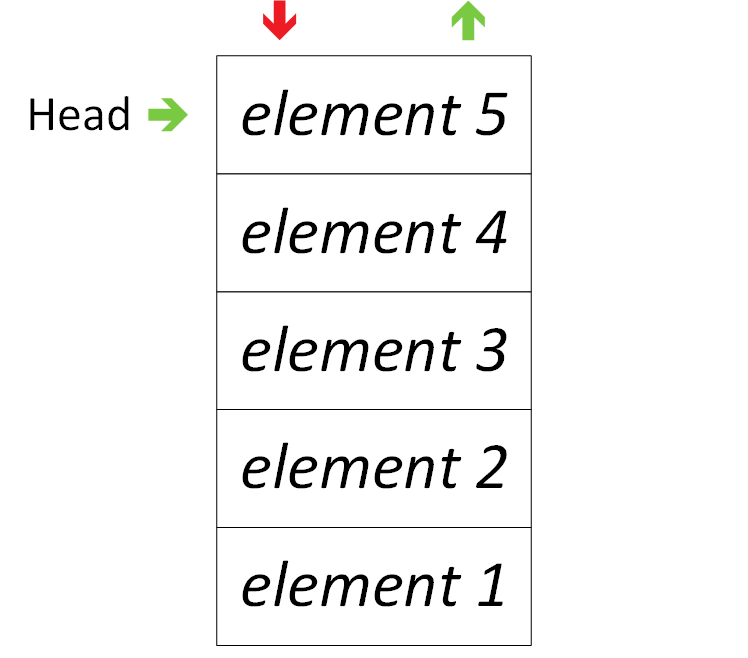
\includegraphics[scale=0.75]{Cours/Piles_1_Structure_Generale_centered.png}
\end{center}

\smallskip

Deux opérations permettent d'utiliser une pile :
\begin{itemize}
\item \TTBF{PUSH} : permettant d'\textit{empiler} une donnée supplémentaire dans la pile
\item \TTBF{POP} : permettant de \textit{dépiler} une donnée depuis la pile
\end{itemize}
On ajoute donc une donnée en l'empilant avec un \TTBF{PUSH}, et il est possible de directement y accéder, car elle est au sommet de la pile.
À l'inverse, pour accéder à une donnée tout au fond de la pile, il est nécessaire de dépiler autant d'éléments que nécessaire avec un \TTBF{POP}.\\

Voici un exemple où l'on crée une pile, puis on empile successivement $ 42 $, $ 5 $, et $ 13 $, puis, on dépile une fois (pour récupérer $ 13 $), et enfin, on empile successivement $ 37 $, $ 10 $, $ 24 $.\\

\begin{center}
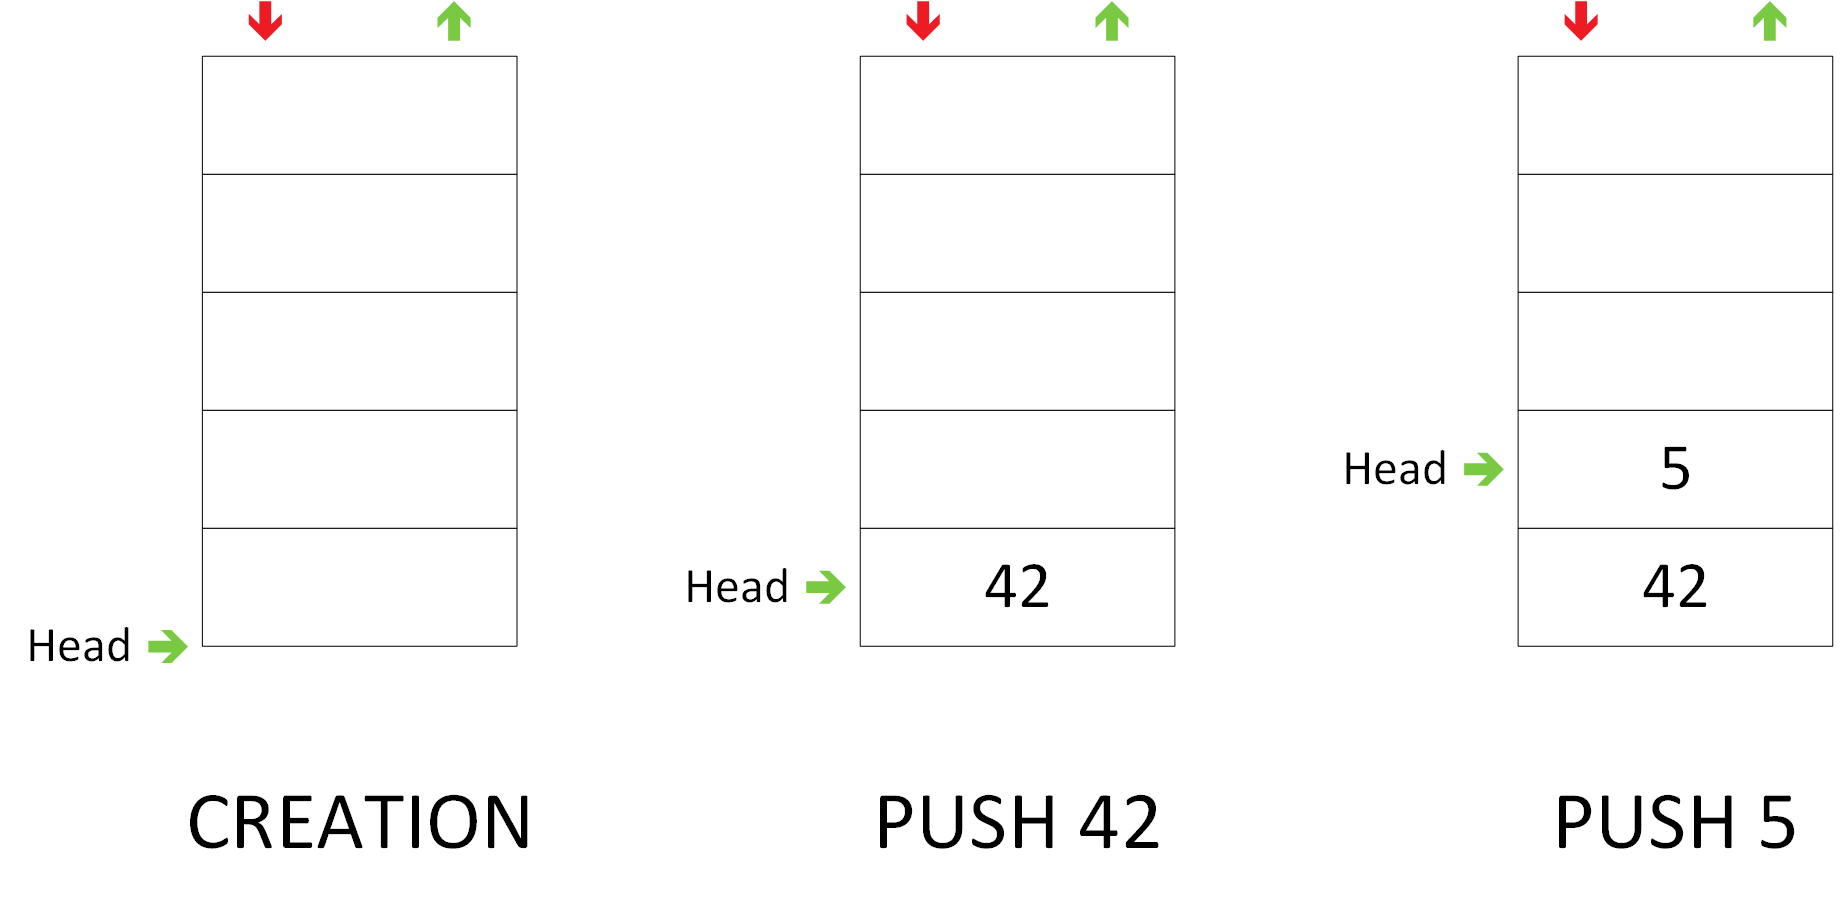
\includegraphics[scale=0.5]{Cours/Piles_2_Structure_Generale_Usage_pack_1.png}
\end{center}

\begin{center}
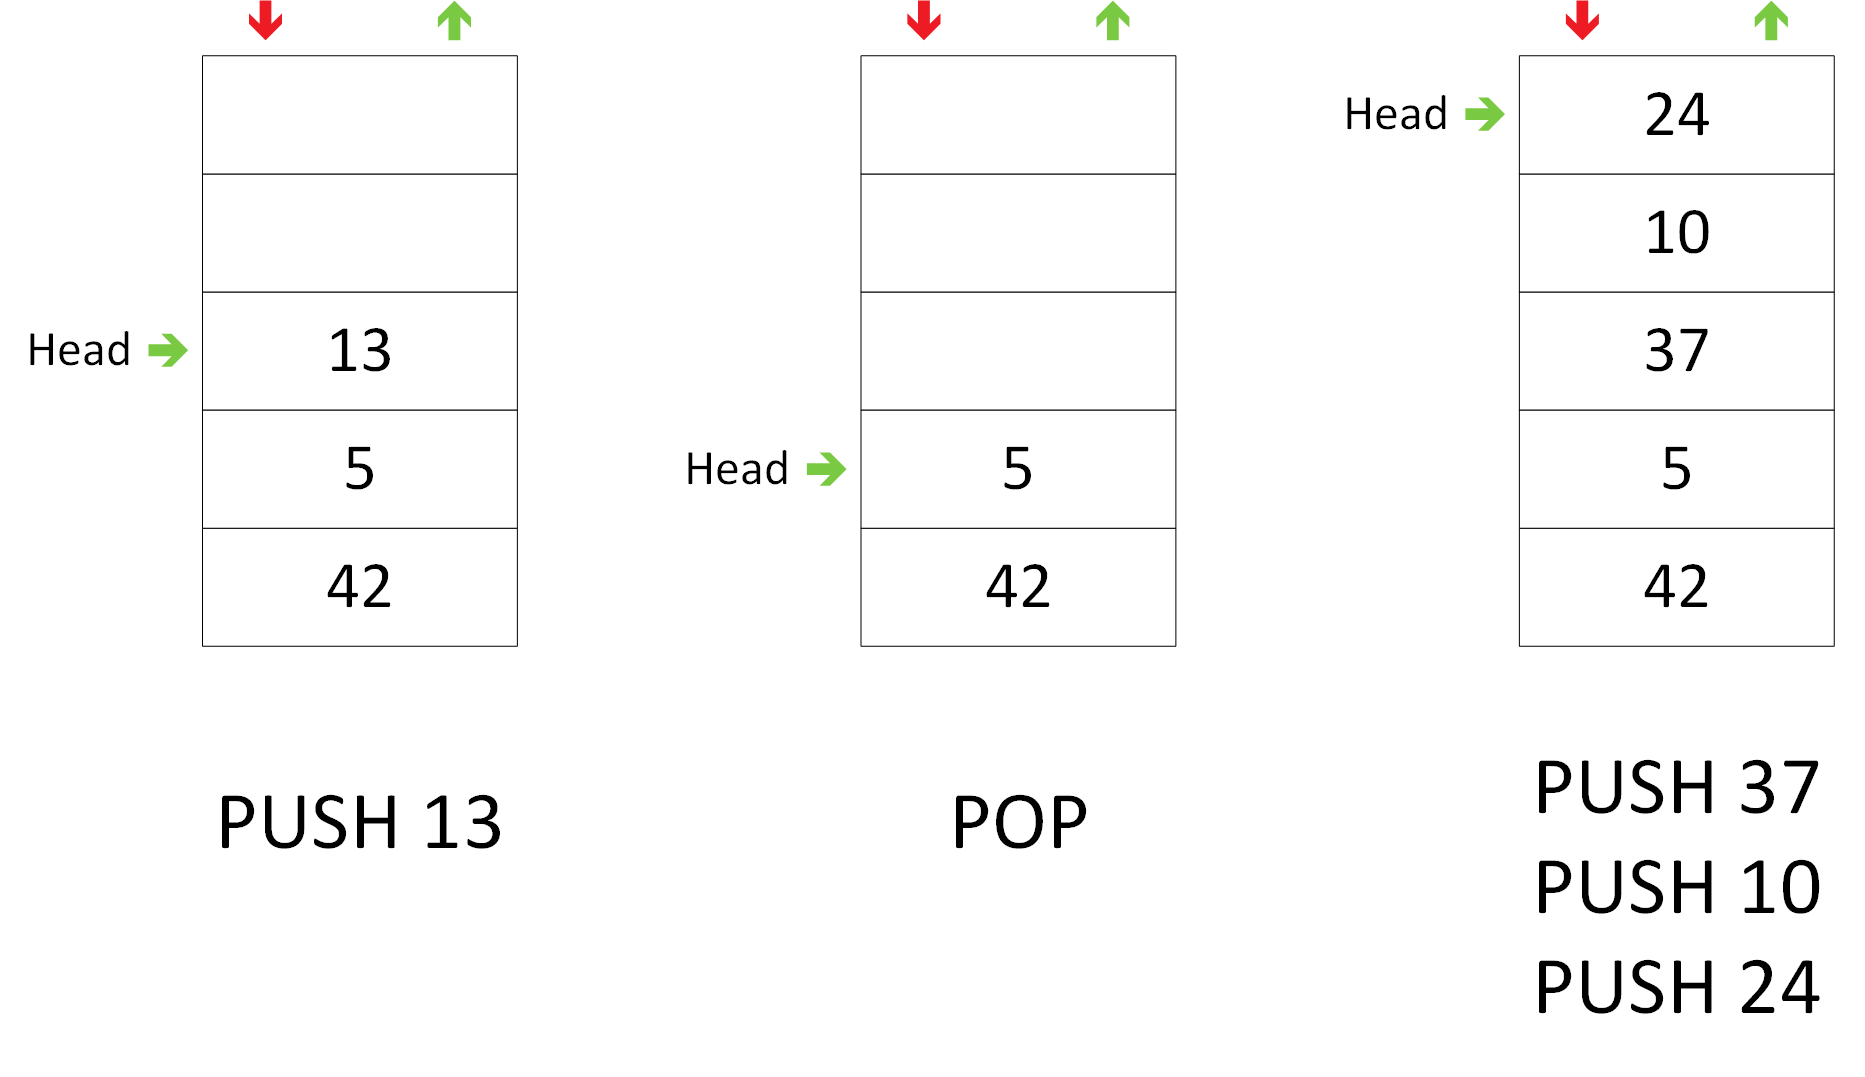
\includegraphics[scale=0.5]{Cours/Piles_2_Structure_Generale_Usage_pack_2.png}
\end{center}

\smallskip

Les piles, et surtout la contrainte d'accès aux objets, sont couramment utilisées : un camion de livraison sera d'abord rempli avec les paquets à livrer en dernier/le camion sera rempli dans l'ordre inverse de livraison (on accède d'abord aux derniers éléments chargés).

En informatique, on utilisera les piles dans certains \textit{parsers} (analyse grammaticale) pour connaître en premier l'opérateur à exécuter (opérateur binaire ? unaire ?) et dépiler par la suite le nombre exact de paramètres.
La \textit{pile d'appels} est également une convention fondamentale partagée par les processeurs et les systèmes d'exploitation permettant de passer des paramètres (et d'autres informations de contexte) aux fonctions appelées par les programmes, ou en cas d'interruption pour sauvegarder l'adresse de l'instruction qui était en cours d'exécution.\\

Afin d'implémenter une pile, il est donc nécessaire d'avoir un espace de stockage ordonné (un tableau numéroté ou une liste chaînée), et un indicateur de l'élément en haut de la pile.
Nous allons maintenant voir comment implémenter une pile avec des listes chaînées et un tableau de taille fixe.

\bigskip

%%%%%%%%%%%%%%%%%%%%%%%%%%%%%%%%%%%%%%%%%%%%%%%%%%%%%%%%%%%%
%%%%%%%%%%%%%%%%%%%%%%%%%%%%%%%%%%%%%%%%%%%%%%%%%%%%%%%%%%%%
%%%%%%%%%%%%%%%%%%%%%%%%%%%%%%%%%%%%%%%%%%%%%%%%%%%%%%%%%%%%

\subsection{Piles : implémentation avec des listes chaînées}

\bigskip

Une implémentation à l'aide d'une liste chaînée permet d'exploiter la mémoire et d'être donc beaucoup plus flexible en terme de nombre maximum d'éléments.
Le schéma suivant illustre une pile sous forme de liste chaînée en mémoire :\\

\begin{center}
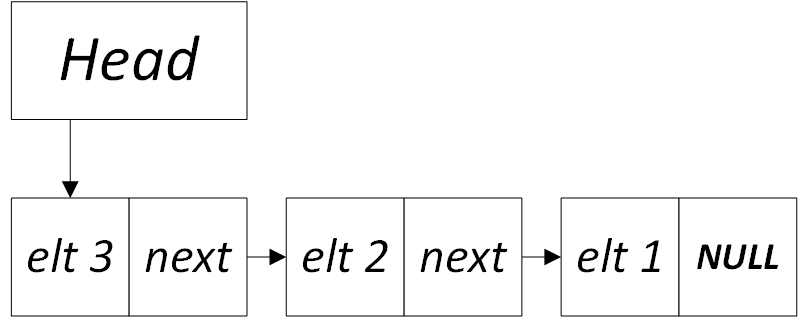
\includegraphics[scale=0.75]{Cours/Piles_3_Liste_Chainee_Structure_cas_general.png}
\end{center}

\smallskip

On y retrouve plusieurs fois la structure typique des listes chaînées (un élément et un pointeur vers l'élément suivant), ainsi qu'un pointeur indiquant le sommet de la pile (\textit{head} dans notre cas).

L'unique cas particulier concerne une pile vide : le pointeur de sommet vaut dans ce cas \TTBF{NULL}.
Il s'agit également de l'état dans lequel se trouve une pile vidée ou nouvellement créée.\\

\begin{center}
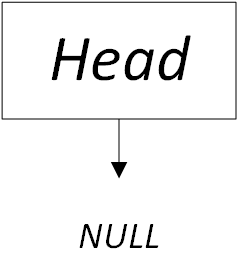
\includegraphics[scale=0.75]{Cours/Piles_3_Liste_Chainee_Structure_cas_vide.png}
\end{center}

\smallskip

L'exemple suivant montre l'évolution d'une pile au fur et à mesure des ajouts (empiler / \TTBF{PUSH}) et suppressions (dépiler / \TTBF{POP}).\\

\begin{center}
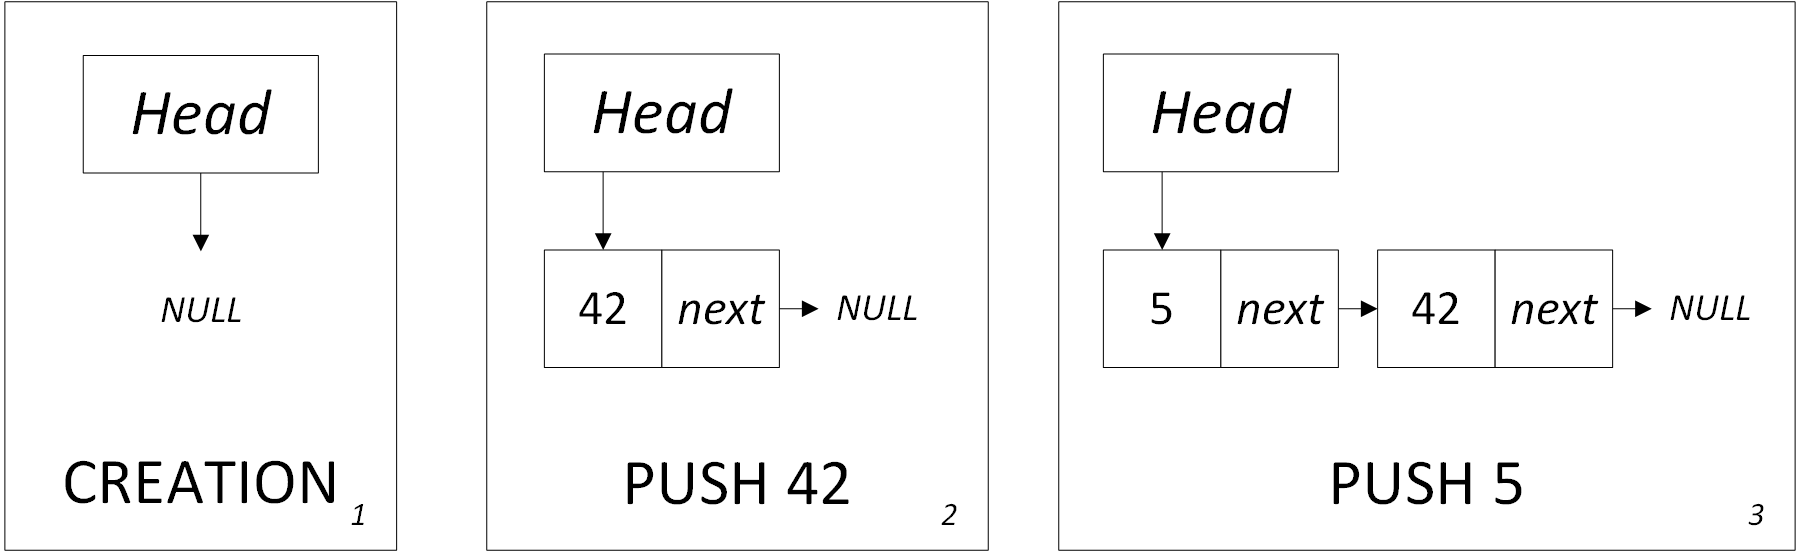
\includegraphics[scale=0.65]{Cours/Piles_4_Liste_Chainee_Usage_pack_1.png}
\end{center}

\begin{center}
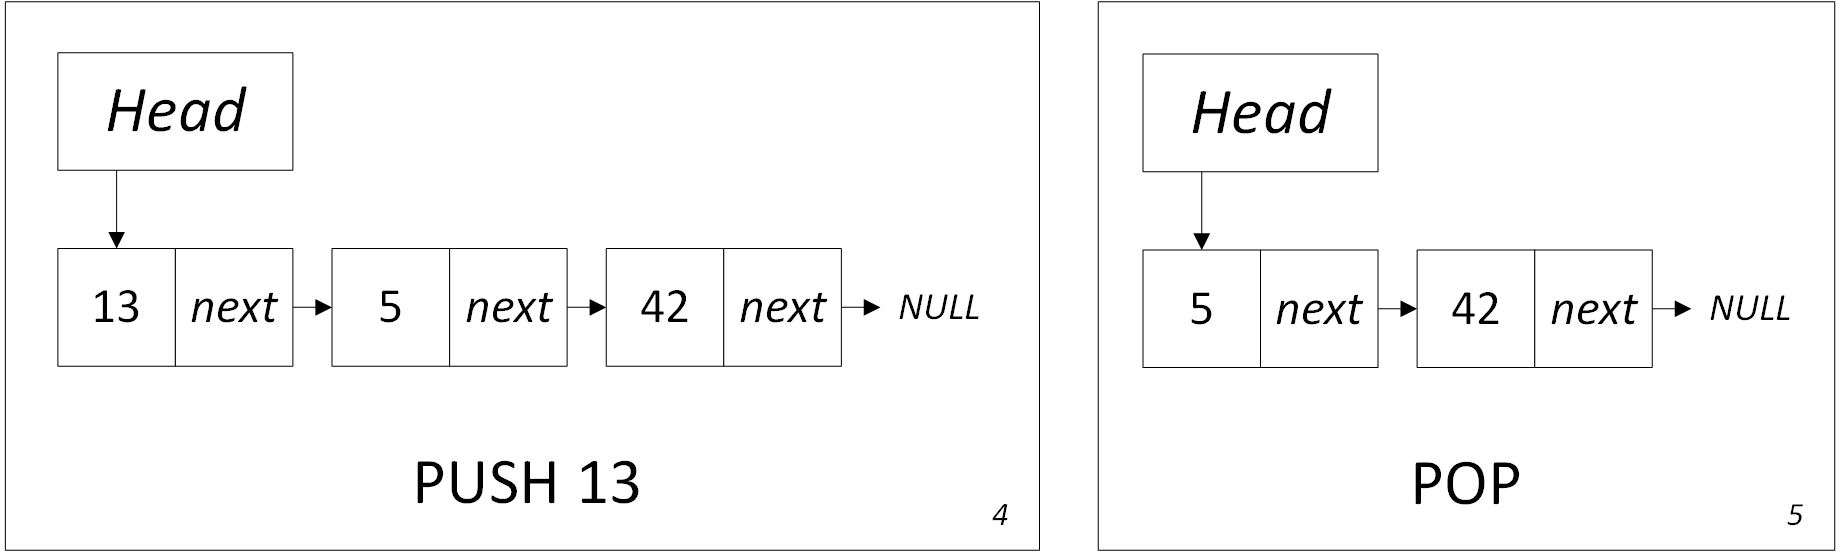
\includegraphics[scale=0.65]{Cours/Piles_4_Liste_Chainee_Usage_pack_2.png}
\end{center}

\smallskip

Les principales opérations se résument ainsi :
\begin{itemize}
\item Création : on alloue en mémoire la structure générale de la pile, et on fixe le sommet de la pile à \TTBF{NULL}.
\item Empiler : on alloue en mémoire un nouvel élément dont le pointeur \textit{next} pointe vers l'actuel élément au sommet de la pile, puis, on met à jour le pointeur de sommet de la pile vers l'adresse de ce nouvel élément.
\item Dépiler : si la pile est vide, on retourne une erreur, sinon, on récupère tout d'abord l'adresse de l'élément suivant celui au sommet, puis, on libère l'élément au sommet, puis, on met à jour le pointeur de sommet de la pile vers l'adresse de l'élément suivant.
\item Vider : on dépile successivement tous les éléments jusqu'à obtenir un sommet à \TTBF{NULL}.
\item Sommet : on renvoie le contenu de l'élément au sommet de la pile.
\end{itemize}

\bigskip

%%%%%%%%%%%%%%%%%%%%%%%%%%%%%%%%%%%%%%%%%%%%%%%%%%%%%%%%%%%%
%%%%%%%%%%%%%%%%%%%%%%%%%%%%%%%%%%%%%%%%%%%%%%%%%%%%%%%%%%%%
%%%%%%%%%%%%%%%%%%%%%%%%%%%%%%%%%%%%%%%%%%%%%%%%%%%%%%%%%%%%

\subsection{Piles : implémentation avec un tableau de taille fixe}

\bigskip

Une implémentation avec un tableau de taille fixe impose cette fois une limitation : la pile aura une taille maximale, et on peut refuser l'ajout d'un élément si la pile est déjà pleine.
La structure diffère également du fait que le tableau est alloué une seule fois lors de sa création (voire même lors de la compilation dans le cas statique).

Le schéma suivant présente la structure générale :\\

\begin{center}
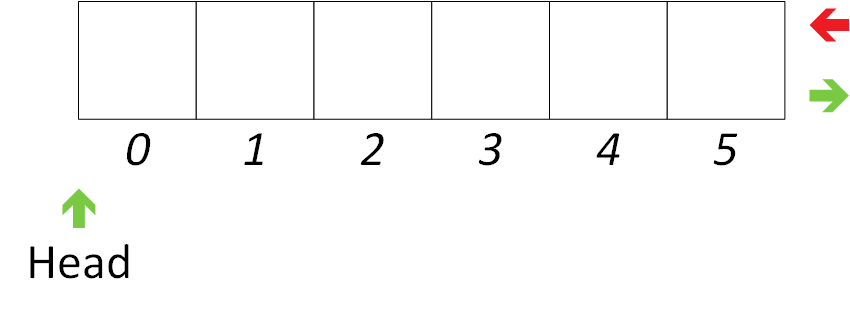
\includegraphics[scale=1]{Cours/Piles_5_Tableau_Statique_Structure.png}
\end{center}

\smallskip

On notera cette fois que plusieurs informations distinctes doivent être conservées : l'adresse du tableau, le numéro de case correspondant au sommet de la pile (\textit{head} dans notre cas), la taille du tableau (le nombre maximum d'objets pouvant être stockés), le nombre d'éléments dans le tableau.

Le schéma suivant détaille certaines informations de façon plus explicite :\\

\begin{center}
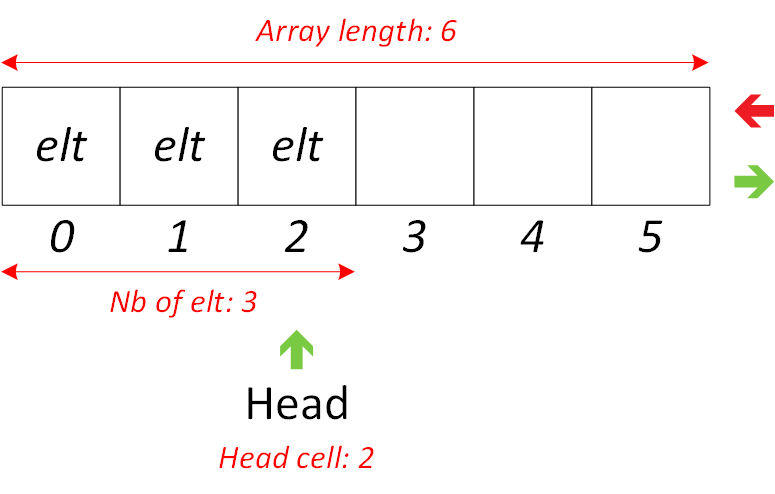
\includegraphics[scale=1]{Cours/Piles_5_Tableau_Statique_Structure_Detaillee.png}
\end{center}

\smallskip

Dans le cas d'un tableau de taille fixe, le pointeur de sommet ne peut pas utiliser la valeur \TTBF{NULL} comme indicateur de tableau vide, car cette valeur est égale à $ 0 $ (ce qui laisserait à penser que le sommet est effectivement à la case 0).
Plusieurs solutions sont possibles pour indiquer le sommet de la pile et le cas vide :

\begin{itemize}
\item On enregistre dans la structure de la pile une variable servant à compter le nombre d'éléments présents (le sommet peut donc prendre n'importe quelle valeur tant que la pile est vide).
\item On utilise un entier relatif pour indiquer le sommet, et $ -1 $ indique que la pile est vide (l'ajout d'un élément décalera le sommet à $ 0 $, c'est-à-dire la case où sera l'élément).
\item On place le sommet de la pile sur la première case non utilisée, et l'accès au premier élément se fait donc en retirant $ 1 $ au pointeur de sommet (ainsi, un sommet à la case $ 0 $ indique que la pile est vide).
Attention : dans ce cas précis, un tableau plein aura un sommet hors des cases du tableau (il ne faudra donc \textit{jamais} le déréférencer s'il atteinte une telle valeur).
\end{itemize}

\smallskip

L'exemple suivant montre l'évolution d'une pile implémentée avec un tableau fixe au fur et à mesure des ajouts (empiler / \TTBF{PUSH}) et suppressions (dépiler / \TTBF{POP}).\\

\begin{center}
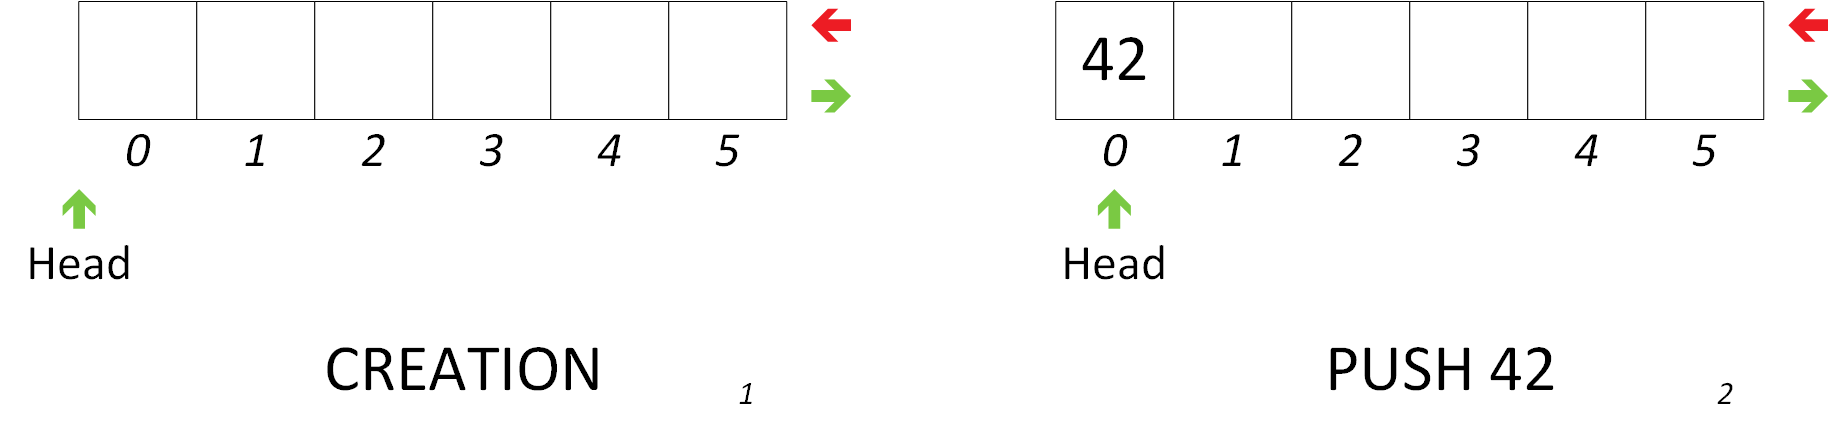
\includegraphics[scale=0.65]{Cours/Piles_6_Tableau_Statique_Usage_pack_1.png}
\end{center}

\begin{center}
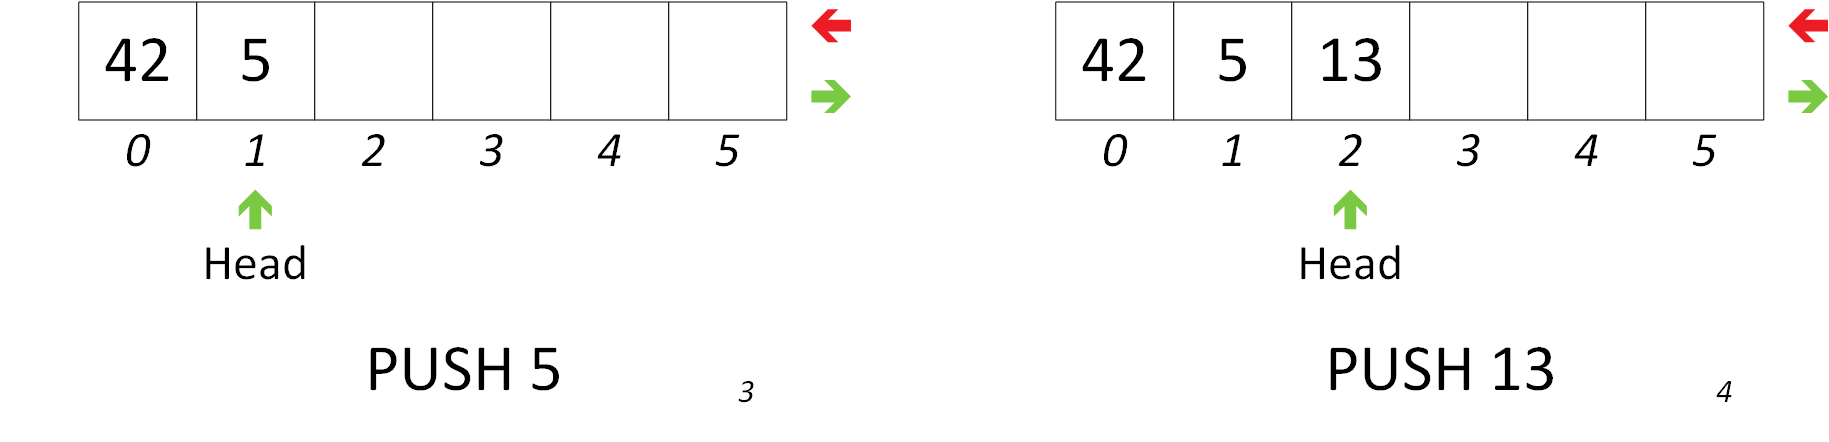
\includegraphics[scale=0.65]{Cours/Piles_6_Tableau_Statique_Usage_pack_2.png}
\end{center}

\begin{center}
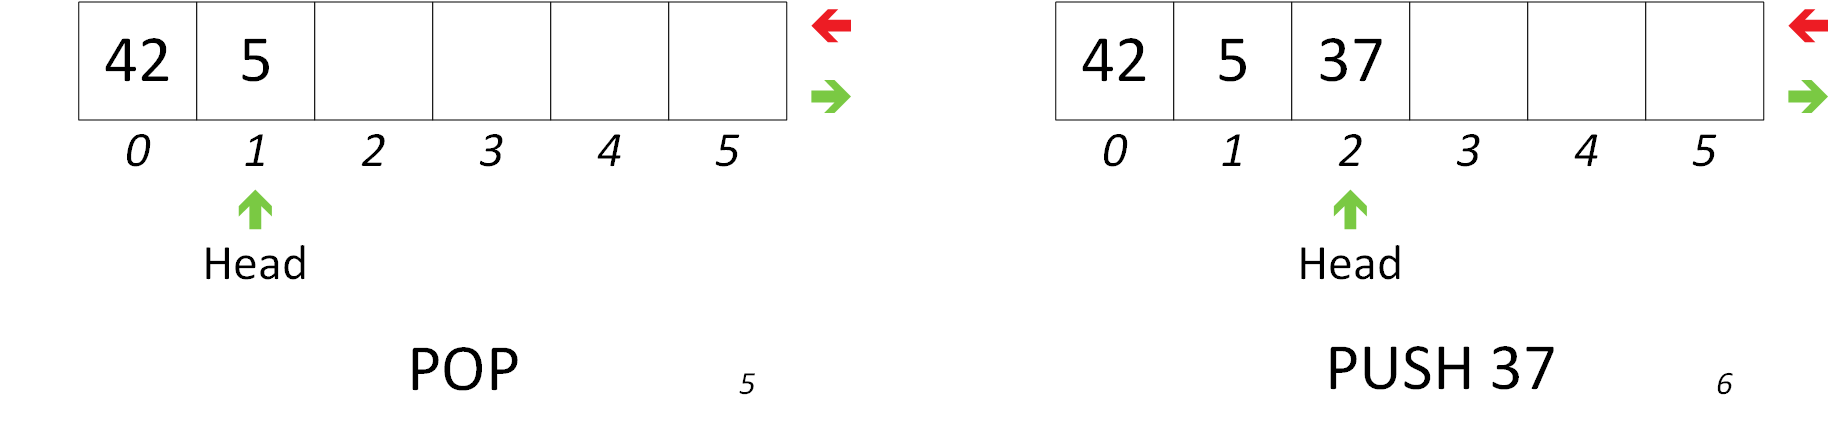
\includegraphics[scale=0.65]{Cours/Piles_6_Tableau_Statique_Usage_pack_3.png}
\end{center}

\smallskip

Les principales opérations se résument ainsi :
\begin{itemize}
\item Création : on alloue en mémoire le tableau (sauf s'il est statique), et on fixe le sommet de la pile à la valeur prévue pour démarrer ($ -1 $, $ 0 $, ou toute autre valeur choisie) [éventuellement, on met à jour le nombre d'objets dans le tableau en le fixant à $ 0 $].
\item Empiler : si le tableau est plein, on retourne une erreur, sinon, on ajoute un élément, et on décale le sommet de la pile [éventuellement, on met à jour le nombre d'objets dans le tableau].
\item Dépiler : si la pile est vide, on retourne une erreur, sinon, on réduit la valeur du sommet de la pile [éventuellement, on met à jour le nombre d'objets dans le tableau].
\item Vider : on fixe le sommet de la pile à la valeur prévue pour démarrer ($ -1 $, $ 0 $, ou toute autre valeur choisie) [éventuellement, on met à jour le nombre d'objets dans le tableau en le fixant à $ 0 $].
\item Sommet : on renvoie le dernier élément ajouté (cela dépend de comment le sommet a été implémenté !).
\end{itemize}

\setlength{\parindent}{\defaultparindent}

%
%\newpage

%%%%%%%%%%%%%%%
%% EXERCICES %%
%%%%%%%%%%%%%%%

%% Exercice 1
\section{Exercice 1 - Module statistiques}

\vspace*{0.7cm}

%% Exercice 1

%\ExoSpecs{\TTBF{CalculTVA.sh}}{\TTBF{\RenduDir/src/exo1/}}{750}{640}{\TTBF{write}}
\ExoSpecsCustom{\TTBF{exo1\_fun.php} [my\_Calculette(int, int, string)]}{\TTBF{\RenduDir/src/exo1/}}{}{}{Fonctions recommandées}{\TTBF{(Bases PHP)}, \TTBF{(Maths PHP)}, \TTBF{return}}

\vspace*{0.7cm}

\noindent \ExoObjectif{Le but de l'exercice est de créer une mini calculatrice en PHP.}

\bigskip

\noindent Vous devez écrire une fonction nommée \TTBF{my\_Calculette} qui prendra trois paramètres (deux nombres, puis l'opérateur), et renverra le résultat de l'opération désignée ou un message d'erreur.

\noindent Vous devez implémenter les 5 opérations suivantes : l'addition (symbole \TTBF{+}), la soustraction (symbole \TTBF{-}), la multiplication (lettre \TTBF{*}), la division (symbole \TTBF{/}), et le reste de la division euclidienne (symbole  \TTBF{\%}).

\noindent \`A la fin du calcul, votre fonction doit renvoyer le résultat.

\bigskip

\lstset{language=php}
\begin{lstlisting}[frame=single,title={Cas général PHP}]
<textarea cols="80" rows="25" readonly="readonly">
<?php
  require_once("exo1_fun.php");
  $my_text = my_Calculette(42, 38, "+");
  echo($my_text);
?>
</textarea>
\end{lstlisting}

\lstset{language=php}
\begin{lstlisting}[frame=single,title={Cas général PHP exécuté}]
<textarea cols="80" rows="25" readonly="readonly">
80</textarea>
\end{lstlisting}

\bigskip

\noindent Les deux premiers paramètres doivent être des entiers, et le troisième doit être une chaîne de caractères. Si ça n'est pas le cas, vous devez renvoyer le texte suivant.

\bigskip

\noindent \TTBF{Incorrect\textvisiblespace parameters\textvisiblespace type}

\bigskip

\lstset{language=php}
\begin{lstlisting}[frame=single,title={Cas d'erreur 1 : mauvais paramètres}]
<textarea cols="80" rows="25" readonly="readonly">
<?php
  require_once("exo1_fun.php");
  $my_text = my_Calculette("+", 38, 42);
  echo($my_text);
?>
</textarea>
\end{lstlisting}

\lstset{language=php}
\begin{lstlisting}[frame=single,title={Cas d'erreur 1 exécuté}]
<textarea cols="80" rows="25" readonly="readonly">
Incorrect parameters type</textarea>
\end{lstlisting}

\bigskip

\noindent Si le troisième paramètre donné n'est ni un \TTBF{+}, ni un \TTBF{-}, ni un \TTBF{*}, ni un \TTBF{/}), ni un \TTBF{\%}, alors vous devez renvoyer le message d'erreur suivant.

\bigskip

\noindent \TTBF{Unknown\textvisiblespace operator}

\bigskip

\lstset{language=php}
\begin{lstlisting}[frame=single,title={Cas d'erreur 2 : opérateur inconnu}]
<textarea cols="80" rows="25" readonly="readonly">
<?php
  require_once("exo1_fun.php");
  $my_text = my_Calculette(42, 38, "A");
  echo($my_text);
?>
</textarea>
\end{lstlisting}

\lstset{language=php}
\begin{lstlisting}[frame=single,title={Cas d'erreur 2 exécuté}]
<textarea cols="80" rows="25" readonly="readonly">
Unknown operator</textarea>
\end{lstlisting}

\bigskip

\noindent Si le deuxième paramètre donné à la division est 0, vous devez renvoyer le message d'erreur suivant.

\bigskip

\noindent \TTBF{Division\textvisiblespace by\textvisiblespace 0\textvisiblespace is\textvisiblespace forbidden}

\bigskip

\lstset{language=php}
\begin{lstlisting}[frame=single,title={Cas d'erreur 3 : division par 0}]
<textarea cols="80" rows="25" readonly="readonly">
<?php
  require_once("exo1_fun.php");
  $my_text = my_Calculette(42, 0, "/");
  echo($my_text);
?>
</textarea>
\end{lstlisting}

\lstset{language=php}
\begin{lstlisting}[frame=single,title={Cas d'erreur 3 exécuté}]
<textarea cols="80" rows="25" readonly="readonly">
Division by 0 is forbidden</textarea>
\end{lstlisting}

\bigskip

%\noindent Si le deuxième paramètre donné au modulo est 0, vous devez renvoyer le message d'erreur suivant.
%
%\bigskip
%
%\noindent \TTBF{Modulo\textvisiblespace 0\textvisiblespace is\textvisiblespace forbidden}
%
%\bigskip
%
%\lstset{language=php}
%\begin{lstlisting}[frame=single,title={Cas d'erreur 3 : division par 0}]
%<textarea cols="80" rows="25" readonly="readonly">
%<?php
%  require_once("exo1_fun.php");
%  $my_text = my_Calculette(42, 0, "%");
%  echo($my_text);
%?>
%</textarea>
%\end{lstlisting}
%
%\lstset{language=php}
%\begin{lstlisting}[frame=single,title={Cas d'erreur 3 exécuté}]
%<textarea cols="80" rows="25" readonly="readonly">
%Modulo 0 is forbidden</textarea>
%\end{lstlisting}
%
%\bigskip

\noindent Si plusieurs des problèmes précédents sont rencontrés simultanément, vous devez les gérer dans cet ordre de priorité : le problème de type en priorité, l'opérateur inconnu en second, et la division par 0 en dernier.

%\noindent Si plusieurs des problèmes précédents sont rencontrés simultanément, vous devez les gérer dans cet ordre de priorité : le problème de type en priorité, l'opérateur inconnu en second, et enfin le modulo ou la division par 0 en dernier.

\bigskip

\lstset{language=php}
\begin{lstlisting}[frame=single,title={Cas d'erreurs}]
<textarea cols="80" rows="25" readonly="readonly">
<?php
  require_once("exo1_fun.php");
  $my_text = my_Calculette("A", 42, 0);
  echo($my_text);
?>
</textarea>
\end{lstlisting}

\lstset{language=php}
\begin{lstlisting}[frame=single,title={Cas d'erreurs exécuté}]
<textarea cols="80" rows="25" readonly="readonly">
Incorrect parameters type</textarea>
\end{lstlisting}

\lstset{language=php}
\begin{lstlisting}[frame=single,title={Cas d'erreurs}]
<textarea cols="80" rows="25" readonly="readonly">
<?php
  require_once("exo1_fun.php");
  $my_text = my_Calculette(42, 0, "A");
  echo($my_text);
?>
</textarea>
\end{lstlisting}

\lstset{language=php}
\begin{lstlisting}[frame=single,title={Cas d'erreurs exécuté}]
<textarea cols="80" rows="25" readonly="readonly">
Unknown operator</textarea>
\end{lstlisting}


\newpage

%% Exercice 2
\section{Exercice 2 - Classe statistiques}

\vspace*{0.7cm}

%% Exercice 2

%\ExoSpecs{\TTBF{CalculTVA.sh}}{\TTBF{\RenduDir/src/exo1/}}{750}{640}{\TTBF{write}}
\ExoSpecsCustom{\TTBF{Makefile}}{\TTBF{\RenduDir/}}{750}{640}{Outils recommandés}{\TTBF{gcc(1)}, \TTBF{ar(1)}}

\vspace*{0.7cm}

\noindent \ExoObjectif{Le but de l'exercice est de faire fonctionner l'ensemble de votre projet avec un makefile simple, et de produire une bibliothèque statique ainsi qu'une dynamique.}

\bigskip

\noindent Une bibliothèque est un ensemble de fonctions et procédures prêtes à être utilisées (ayant éventuellement des variables statiques, ou encore faisant appel à \texttt{malloc(3)}) par un utilisateur ne connaissant pas leur implémentation.
L'utilisateur développe et écrit son propre programme (utilisant un \texttt{main} pour s'exécuter) et il peut éventuellement s'appuyer sur des bibliothèques (n'ayant pas de \texttt{main}) pour réutiliser des implémentations existantes.

\bigskip

\noindent Les exercices suivants vont vous conduire à produire des fonctions manipulant des structures, afin d'offrir un service à des utilisateurs : des arbres binaires et leur interface pour les exploiter (une \texttt{API}).
Vous devez donc écrire le (ou les) \textit{makefile(s)} de votre projet et un fichier \texttt{configure} (éventuellement vide) afin de produire une bibliothèque statique nommée \TTBF{libmybintree.a} et une bibliothèque dynamique nommée \TTBF{libmybintree.so}.

\bigskip

\noindent Le \textit{makefile} que vous allez écrire rendra votre projet complet et autonome.
Pour cela, vous devez faire en sorte que plusieurs \textit{cibles} soient présentent dans le makefile (celles-ci sont rappelées dans le paragraphe suivant).
%Afin de rendre le projet parfaitement complet et autonome, vous devez écrire un \textit{makefile} répondant aux cibles indiquées dans les consignes générales (celles-ci sont rappelées dans le paragraphe suivant).

\bigskip

\noindent Plusieurs stratégies existent pour compiler avec des makefiles, l'une d'entre elle consiste à placer un makefile par dossier afin que le makefile principal appelle les suivants avec la bonne règle (par exemple : le makefile principal va appeler le makefile du dossier \textit{src} pour compiler le projet, mais le makefile principal appellera celui du dossier \textit{check} lorsque l'on demandera d'exécuter la suite de tests).

\noindent Pour ce premier contact avec les makefiles, vous pouvez vous contenter d'un seul makefile à la racine exécutant des lignes de compilation toutes prêtes sans aucune réécriture ou extension.

\bigskip

\noindent Afin de générer des bibliothèques statiques et dynamiques, vous devez compiler vos fichiers pour produire des fichiers \textit{objets} (des fichiers \TTBF{.o}), mais vous ne devez pas laisser l'étape d'\textit{édition de liens} classique se faire.
À la place, la cible \textit{static} de votre makefile devra produire une bibliothèque statique nommée \TTBF{libmybintree.a}, et la cible \textit{shared} devra produire une bibliothèque dynamique nommée \TTBF{libmybintree.so}.

\bigskip

\noindent Pour générer une bibliothèque statique (\textit{static library} en anglais), on utilise la commande \TTBF{ar} qui créée des \textit{archives}.
Pour produire la bibliothèque statique \textit{libtest.a} à partir des fichiers \textit{test1.c} et \textit{file.c}, on utilisera ces commandes :\\

\begin{tabular}{l}
\TTBF{cc -c test1.c file.c}\\
\TTBF{ar cr libtest.a test1.o file.o}\\
\end{tabular}

\bigskip

\noindent Pour générer une bibliothèque dynamique (\textit{shared library} en anglais), on utilise l'option \TTBF{-shared} du compilateur.
Pour produire la bibliothèque dynamique \textit{libtest.so} à partir des fichiers \textit{test1.c} et \textit{file.c}, on utilisera ces commandes :\\

\begin{tabular}{l}
\TTBF{cc -c test1.c file.c} \\
\TTBF{cc test1.o file.o -shared -o libtest.so} \\
\end{tabular}

\bigskip

\noindent La première commande génère des fichiers objets, et la deuxième les réunit dans un seul fichier.
Il arrivera sur certains systèmes qu'il soit nécessaire d'ajouter l'option \TTBF{-fpic} ou \TTBF{-fPIC} (\textit{Position Independent Code}) pour générer des bibliothèques dynamiques.
Gardez en tête que \textit{toutes} les bibliothèques \textbf{doivent} être préfixées par un \textit{\texttt{lib}} dans le nom des fichiers \TTBF{.a} et \TTBF{.so} générés.
Mais, lorsque l'on utiliser une bibliothèque dans un projet, on doit ignorer ce préfixe lors de la compilation et l'édition de liens.

\bigskip

\noindent Pour utiliser une bibliothèque dynamique sur votre système, plusieurs méthodes existent selon le système où vous vous trouvez.\\

\begin{itemize}
\item L'une d'entre elle consiste à ajouter le dossier contenant la bibliothèque à la variable d'environnement \TTBF{LD\_LIBRARY\_PATH} (comme pour la variable \TTBF{PATH}).
Selon votre système, il peut s'agir de la variable d'environnement \TTBF{DYLD\_LIBRARY\_PATH}, \TTBF{LIBPATH}, ou encore \TTBF{SHLIB\_PATH}.
Pour ajouter le dossier courant comme dossier contenant des bibliothèques dynamiques en plus d'autres dossiers, vous pouvez taper :\\
\TTBF{export LD\_LIBRARY\_PATH=.:/usr/lib:/usr/local/lib}
\\

\item Une autre méthode consiste à modifier le fichier \TTBF{/etc/ls.so.conf} et/ou ajouter un fichier contenant le chemin vers votre bibliothèque dans \TTBF{/etc/ld.so.conf.d/} puis à exécuter \TTBF{/sbin/ldconfig} pour recharger les dossiers à utiliser.\\

\item Enfin, vous pouvez demander les droits administrateur et installer votre bibliothèque dans \TTBF{/usr/lib} ou \TTBF{/usr/local/lib}.\\
\end{itemize}

\bigskip

\noindent \'Evidemment, à long terme, l'objectif est d'avoir une bibliothèque installée dans le répertoire \TTBF{/usr/lib}.
Mais, lors du développement, il est préférable d'utiliser la variable \TTBF{LD\_LIBRARY\_PATH}.
Pour vous assurer du fonctionnement de votre exécutable, vous pouvez utiliser \TTBF{ldd(1)} avec le chemin complet vers un exécutable.
\TTBF{ldd} vous indiquera quelles bibliothèques sont requises, et où celui-ci les trouve.
Si l'une d'entre elle n'est pas trouvée, \TTBF{ldd} vous en informera :\\

\TTBF{ldd /usr/bin/ls}

\TTBF{ldd my\_main}


\bigskip

\noindent Pour rappel voici les cibles demandées pour le \TTBF{Makefile} principal à la racine de votre projet :

\bigskip

\begin{table}
%\centering
\begin{tabular}{l p{12cm}}
\texttt{all} & \textit{[Première règle]} lance la règle \texttt{libmybintree}.\\
\texttt{clean} & supprime tous les fichiers temporaires et ceux créés par le compilateur.\\
\texttt{dist} & crée une archive propre, valide, et répondant aux exigences de rendu.\\
\texttt{distclean} & lance la règle \texttt{clean}, puis supprime les binaires et bibliothèques.\\
\texttt{check} & lance le(s) script(s) de test.\\
\texttt{libmybintree} & lance les règles \texttt{shared} et \texttt{static} \\
\texttt{shared} & compile l'ensemble du projet avec les options de compilations exigées et génère une bibliothèque dynamique.\\
\texttt{static} & compile l'ensemble du projet avec les options de compilations exigées et génère une bibliothèque statique.\\
\end{tabular}
\end{table}

\phantom{42}

\vfillFirst

\vfillLast


\newpage

%% Définitions et exemples
\section{Formules statistiques}

\vspace*{0.7cm}


\subsection{Cardinal}

\noindent Le \textit{cardinal} est le nombre de valeurs contenues dans une distribution.

\begin{center}
\begin{equation*}
\text{Nombre de Valeurs} = \text{cardinal de la distribution} = \text{\textit{card}}(L) = |L|
\end{equation*}
\end{center}


\bigskip


\subsection{\'Etendue}

\noindent L'\textit{étendue} est la différence entre la plus grande valeur de la distribution et la plus petite valeur de la distribution.

\begin{center} % \text{étendue} = \text{Valeur}_{\text{\textit{max}}} - \text{Valeur}_{\text{\textit{min}}}
\begin{equation*}
\text{étendue} = E = \text{\textit{max}}(L) - \text{\textit{min}}(L)
\end{equation*}
\end{center}


\bigskip


\subsection{Moyenne}

\noindent La \textit{moyenne arithmétique}, communément appelée \textit{moyenne}, est la somme de tous les éléments de la distribution divisée par le cardinal.

\begin{center} % \text{moyenne} = \frac{\sum_{n=1}^{\text{Nb Valeurs}} \text{Valeur}_{i}}{\text{Nb Valeurs}}
\[
\text{moyenne} = \mu = \bar{L} = \frac{\displaystyle \sum L_{i}}{|L|}
\]
\end{center}

% DistrNbValues = 10
% moyenne = 0
% for (x in range(0, DistrNbValues)):
%   valeur = int(random.random() * 100)
%   moyenne += valeur
% moyenne = moyenne / DistrNbValues


\bigskip


\subsection{Médiane}

\noindent La \textit{médiane} est la valeur centrale d'une distribution triée.

\begin{itemize}
\item En cas de quantité impaire de valeurs, on prend la valeur à la position $ \frac{n + 1}{2} $.
\item En cas de quantité paire de valeurs, on prend la moyenne des deux valeurs centrales.
\end{itemize}

\begin{center} % \text{médiane} = \text{Valeur}_{\frac{i}{\text{Nb Valeurs}}}
\begin{equation*}
\text{médiane} = L_{\frac{|L|}{2}}
\end{equation*}
\end{center}

\bigskip

\noindent Par exemple pour la distribution suivante : 4 5 6

\noindent La médiane sera de $ 5 $, car $ \frac{3 + 1}{2} = 2 $ et $ 5 $ et le deuxième nombre de la distribution.

\bigskip

\noindent Par exemple pour la distribution suivante : 1 2 3 4

\noindent La médiane sera de $ 2,5 $, car $ 2 $ et $ 3 $ sont les valeurs centrales et $ \mu(2 ; 3) = 2,5 $.

\bigskip

\noindent \textbf{\textit{Attention : n'oubliez pas que Python compte depuis 0 pour la position dans les listes.}}

% import math
% median_pos = int(math.floor(DistrNbValues / 2))
% sorted_distr = MyDistribution.copy()
% sorted_distr.sort()
% median = sorted_distr[median_pos]


\bigskip


\subsection{Quartiles et \'Ecart interquartiles}

\subsubsection{Quartiles}

\noindent L'\textit{écart interquartile} est basé sur la différence entre des \textit{quartiles}.
L'idée des quartiles est de diviser la distribution en $ 4 $ parties, chaque quartile étant un séparateur, et d'observer l'écart entre certains séparateurs pour mesurer la dispersion des valeurs.

\bigskip

\begin{itemize}
\item le quartile 0 ($Q_{0}$) est la valeur la plus petite de la distribution
\item le $ 1^{er} $ quartile ($Q_{1}$) sépare les $ 25\% $ premières valeurs de la distribution des autres
\item le $ 2^{\grave{e}me} $ quartile ($Q_{2}$) sépare les $ 50\% $ premières valeurs de la distribution des autres
\item le $ 3^{\grave{e}me} $ quartile ($Q_{3}$) sépare les $ 75\% $ premières valeurs de la distribution des autres
\item le quartile 4 ($Q_{4}$) est la valeur la plus élevée de la distribution
\end{itemize}

\bigskip

\noindent Plus visuellement, la distribution triée est séparée ainsi :

\begin{center}
$ Q_{0} $ ... (partie 1) ... $ Q_{1} $ ... (partie 2) ... $ Q_{2} $ ... (partie 3) ... $ Q_{3} $ ... (partie 4) ... $ Q_{4} $
\end{center}

\bigskip

\noindent Dans le cas dit \textit{discret} (c'est-à-dire non continu : on peut dénombrer les valeurs que l'on étudie), il n'existe pas une seule méthode universellement acceptée...
Vous implémenterez donc celle de Wikipédia (en français au 20 août 2023) décrite par la suite :
Il suffit de calculer le \textit{rang} des valeurs, c'est-à-dire leur position dans la distribution triée par ordre croissant.
Un quartile dans le cas discret est donc simplement une valeur à une position précise dans la distribution triée.

\bigskip

\noindent Pour une distribution contenant $ n $ valeurs, on calcule les rangs ainsi :

\begin{itemize}
\item le quartile 0 ($Q_{0}$) est donc au rang $ 1 $
\item le $ 1^{er} $ quartile ($Q_{1}$) est au rang $ (n + 3) / 4 $
\item le $ 2^{\grave{e}me} $ quartile ($Q_{2}$) est au rang $ (n + 1) / 2 $ \textit{(il s'agit de la médiane)}
\item le $ 3^{\grave{e}me} $ quartile ($Q_{3}$) est au rang $ (3n + 1) / 4 $
\item le quartile 4 ($Q_{4}$) est donc au rang $ n $
\end{itemize}

\bigskip

\noindent Testons sur la distribution : $ 10 \; 20 \; 30 \; 40 \; 50 \; 60 \; 70 \; 80 \; 90 $

\begin{itemize}
\item $ Q_{0} = L_{1} = 10 $
\item $ Q_{1} = L_{3} = 30 $
\item $ Q_{2} = L_{5} = 50 $
\item $ Q_{3} = L_{7} = 70 $
\item $ Q_{4} = L_{9} = 90 $
\end{itemize}

\bigskip

\noindent La première partie contient donc les valeurs de $ 10 \; 20 \; 30 $, la deuxième partie les valeurs de $ 30 \; 40 \; 50 $, la troisième partie les valeurs $ 50 \; 60 \; 70 $, et la quatrième partie les valeurs $ 70 \; 80 \; 90 $.

\bigskip

\noindent Testons maintenant sur la distribution : $ 10 \; 20 \; 30 \; 40 \; 50 \; 60 \; 70 \; 80 $

\begin{itemize}
\item $ Q_{0} = L_{1} = 10 $
\item $ Q_{1} = L_{2,75} = ?? $
\item $ Q_{2} = L_{4,5}  = ?? $
\item $ Q_{3} = L_{6,25} = ?? $
\item $ Q_{4} = L_{8} = 80 $
\end{itemize}

\bigskip

%Si on ne tombe pas sur un rang précis, il est normalement nécessaire de calculer un poids entre la valeur au dessus et la valeur au dessous.
%Mais pour simplifier notre cas, utilisons le rang inférieur (avec \TTBF{math.floor}).
%Si on ne tombe pas sur un entier pour le rang, on effectue la moyenne entre le rang inférieur (avec \TTBF{math.floor}) et le rang supérieur (avec \TTBF{math.ceil}) exactement comme lors du calcul de la médiane.
\noindent Si on ne tombe pas sur un entier pour le rang, on effectue la moyenne entre le rang inférieur et le rang supérieur en affectant des poids :

\bigskip

\begin{itemize}
\item si le reste après la virgule est à $ 0,25 $ : on affecte le poids $ 3 $ au rang inférieur, et le poids $ 1 $ au rang supérieur
\end{itemize}
\vspace*{-1cm}
\begin{center}
\[ \scalebox{1.15}{$\displaystyle Q_{X} = \frac{3 * L_{n - 1} \; + \; 1 * L_{n + 1}}{3 \; + \; 1} $} \]
\end{center}

\begin{itemize}
\item si le reste après la virgule est à $ 0,5 $ : on affecte le poids $ 1 $ au rang inférieur, et le poids $ 1 $ au rang supérieur (cela revient à la moyenne des deux)
\end{itemize}
\vspace*{-1cm}
\begin{center}
\[ \scalebox{1.15}{$\displaystyle Q_{X} = \frac{1 * L_{n - 1} \; + \; 1 * L_{n + 1}}{1 \; + \; 1} $} \]
\end{center}

\begin{itemize}
\item si le reste après la virgule est à $ 0,75 $ : on affecte le poids $ 1 $ au rang inférieur, et le poids $ 3 $ au rang supérieur
\end{itemize}
\vspace*{-1cm}
\begin{center}
\[ \scalebox{1.15}{$\displaystyle Q_{X} = \frac{1 * L_{n - 1} \; + \; 3 * L_{n + 1}}{1 \; + \; 3} $} \]
\end{center}

\bigskip

\noindent Reprenons la distribution : $ 10 \; 20 \; 30 \; 40 \; 50 \; 60 \; 70 \; 80 $

\begin{flalign*}
& \scalebox{1.15}{$Q_{0} = L_{1} = 10$} \\
& \scalebox{1.15}{$Q_{1} = L_{2,75} = \frac{1 * L_{2} \; + \; 3 * L_{3}}{1 \; + \; 3} = \frac{1 * 20 + 3 * 30}{1 + 3} = \frac{110}{4} = 27,5$} \\
& \scalebox{1.15}{$Q_{2} = L_{4,5}  = \frac{1 * L_{4} \; + \; 1 * L_{5}}{1 \; + \; 1} = \frac{1 * 40 + 1 * 50}{1 + 1} = \frac{90}{2} = 45$} \\
& \scalebox{1.15}{$Q_{3} = L_{6,25} = \frac{3 * L_{6} \; + \; 1 * L_{7}}{3 \; + \; 1} = \frac{3 * 60 + 1 * 70}{3 + 1} = \frac{250}{4} = 62,5$} \\
& \scalebox{1.15}{$Q_{4} = L_{8} = 80$} \\
\end{flalign*}


% Q0 = 1
% Q1 = (DistrNbValues + 3) / 4
% Q2 = DistrNbValues / 2
% Q3 = ((3 * DistrNbValues) + 1) / 4
% Q4 = DistrNbValues

\bigskip


\subsubsection{\'Ecart interquartile}

\noindent L'\textit{écart interquartile} ou \textit{étendue interquartile} (ou \textit{interquartile range} en anglais et son acronyme \textit{IQR}) est simplement la différence entre le quartile 3 et le quartile 1.

\begin{center} % \text{étendue} = \text{Valeur}_{\text{\textit{max}}} - \text{Valeur}_{\text{\textit{min}}}
\begin{equation*}
\text{écart interquartile} = EI = Q_{3} - Q_{1}
\end{equation*}
\end{center}

% EI = Q3 - Q1


\bigskip


\subsection{Variance}

\noindent La \textit{variance} permet de mesurer la dispersion des valeurs de la distribution par rapport à la moyenne.
L'interprétation est simple : une variance élevée indique que les nombres de la distribution sont éloignés de la moyenne ($ 1 $ et $ 99 $ par rapport à $ 50 $), une variance faible indique que les nombres de la distribution sont proches de la moyenne ($ 42 $ et $ 58 $ par rapport à $ 50 $).
Ici, nous implémenterons la variance d'une population complète, et non pas juste d'un échantillon.

% \frac{\displaystyle (\sum E_{i}^{2}) - \frac{\displaystyle (\sum E_{i})^{2}}
%                                             {\displaystyle \text{Nb Valeurs}}}
%      {\displaystyle \text{Nb Valeurs}}

\begin{center}
\begin{equation*}
\text{variance} = \sigma^{2} = Var(L) = \frac{1}{|L|} \sum (L_{i} - \bar{L})^{2}
\end{equation*}
\end{center}

\bigskip

\noindent Ce calcul peut paraître rebutant, mais il est très simple lorsque l'on regarde de plus près chaque partie de l'expression :

\medskip

\begin{itemize}
\item[$\bullet$] $ (L_{i} - \bar{L}) $ correspond à la différence entre chaque élément de la distribution et la moyenne de la distribution.

\item[$\bullet$] $ (L_{i} - \bar{L})^{2} $ correspond au carré de la différence entre chaque élément de la distribution et la moyenne de la distribution.

\item[$\bullet$] $ \sum (L_{i} - \bar{L})^{2} $ correspond à la somme des carrés précédemment décrits. Il s'agit donc de faire une boucle effectuant les traitements précédemment décrits, pour ajouter le résultat à une variable initialisée à $ 0 $ juste avant la boucle.

\item[$\bullet$] $ \frac{1}{|L|} \sum (L_{i} - \bar{L})^{2} $ correspond à la division par le nombre d'éléments de la distribution du total de la somme précédente.
\end{itemize}

%def Variance1(MyDistribution):
%  DistrNbValues = length(MyDistribution)
%  Moyenne = 0
%  for x in MyDistribution:
%    Moyenne = Moyenne + x
%  Moyenne = Moyenne / DistrNbValues
%  tmp = 0
%  for x in MyDistribution:
%    tmp = tmp + ((x - Moyenne) ** 2)
%  variance = tmp / DistrNbValues
%  return (variance)

\bigskip

\noindent En développant le calcul, on peut arriver à une formule beaucoup plus adaptée au développement, surtout avec des distributions extrêmement grandes (c'est-à-dire des distributions sur lesquelles il coûterait très/trop cher de passer plusieurs fois pour calculer tout d'abord la \textit{moyenne}, et seulement ensuite la différence de chaque élément avec la moyenne), ou lorsque les valeurs arrivent au fur et à mesure sans savoir précisément quand la distribution s'arrêtera (et que l'on souhaite un aperçu des statistiques en temps réel) :

\begin{center}
\begin{equation*}
\text{variance} = \sigma^{2} = Var(L) = \frac{1}{|L|} \sum (L_{i} - \bar{L})^{2} = \left( \frac{1}{|L|} \sum L_{i}^{2} \right) - \bar{L}^{2}
\end{equation*}
\end{center}

\bigskip

\noindent Analysons cette deuxième formule pour comprendre son intérêt en tant que développeur :

\medskip

\begin{itemize}
\item[$\bullet$] $ L_{i}^{2} $ correspond à la mise au carré de chaque élément de la distribution.

\item[$\bullet$] $ \sum L_{i}^{2} $ correspond à la somme de tous les éléments de la distribution mis au carré individuellement, c'est-à-dire d'itérer sur chaque élément, en faire son propre carré, puis d'ajouter ce résultat à une variable mise à $ 0 $ juste avant la boucle.

\item[$\bullet$] $ \frac{1}{|L|} \sum L_{i}^{2} $ correspond à la division de la somme précédente par le nombre d'éléments de la distribution.

\item[$\bullet$] $ ( \frac{1}{|L|} \sum L_{i}^{2} ) - \bar{L}^{2} $ correspond à la différence entre la division précédente, et la moyenne de la distribution mise au carré.
\end{itemize}

\noindent Cette deuxième formule est en réalité bien plus efficace dans un contexte séquentiel (c'est-à-dire lorsque chaque opération est effectuée l'une après l'autre), car nous pouvons faire une somme de tous les éléments qui arrivent et une somme de chacun de leur carré, et seulement lorsque tous les nombres ont été analysés, nous pouvons en déduire la moyenne et la soustraire.
Chaque élément n'aura été lu qu'une seule et unique fois lorsqu'il a été généré, et nous avons fait évolué deux variables distinctes à côté : une somme simple (pour produire la moyenne), et une somme des carrés.

%sumelt = 0
%sumsqelt = 0
%DistrNbValues = N
%
%def Generation(N):
%  for x in range(0, N):
%    elt = random.randint()
%    sumelt = sumelt + elt
%    sumsqelt = sumsqelt + (elt ** 2)
%  ...
%
%def Variance2(MyDistribution):
%  variance = (sumsqelt - ((sumelt ** 2) / DistrNbValues) / DistrNbValues)
%  return (variance)


\bigskip


\subsection{\'Ecart type}

\noindent L'\textit{écart type} (ou \textit{standard deviation} en anglais) permet de mesurer la dispersion d'une distribution.
Plus la mesure est élevée, plus la distribution contient des valeurs éloignées ($ 3 $ et $ 90 $), et plus la mesure est faible, plus la distribution contient des valeurs proches ($ 42 $ et $ 46 $).
On peut comparer les écarts types de distributions issues de mêmes choses (par exemple, les écarts types de plusieurs classes composées d'étudiants).
Ici, nous implémenterons l'écart type d'une population complète, et non pas juste d'un échantillon.

\begin{center}
\begin{equation*}
\text{écart type} = \sigma = \sqrt{Var(L)}
\end{equation*}
\end{center}

% import math
% stddev = math.sqrt(Variance1(MyDistribution))


\bigskip


\subsection{Coefficient de variation/\'Ecart type relatif}

\noindent Le \textit{coefficient de variation} ou \textit{écart type relatif} (ou \textit{relative standard deviation} en anglais et son acronyme \textit{RSD}) permet de mesurer la dispersion d'une distribution autour de la moyenne en générant un pourcentage indépendant des objets étudiés par la distribution.
Plus le pourcentage est faible, plus la distribution est concentrée autour de sa moyenne, plus le pourcentage est élevé, plus la distribution est étalée loin de sa moyenne.
Cependant, l'écart type relatif ne fonctionne pas lorsque la moyenne est proche de $ 0 $ : celui-ci va tendre vers l'infini (donc dépasser les $ 100\% $) et sera très sensible aux variations.
Ici, nous implémenterons l'écart type relatif d'une population complète, et non pas juste d'un échantillon.

\begin{center}
\begin{equation*}
\text{coefficient de variation} = c_{v} = \frac{\sigma}{\mu} = \frac{\sqrt{Var(L)}}{\bar{L}}
\end{equation*}
\end{center}

% import math
% stddev = math.sqrt(Variance1(MyDistribution))
% RSD = stddev / mean(MyDistribution)


\bigskip


\subsection{Coefficient de Gini}

\noindent Le \textit{coefficient de Gini} est un indice particulièrement utilisé dans le monde économique et social.
Ce coefficient a été constitué pour mesurer les inégalités de revenus au sein d'une population, mais il permet plus généralement de mesurer l'inégalité de répartition d'une variable (donc son interprétation s'approche des mesures de dispersion).
Le coefficient de Gini calcule une valeur entre $ 0 $ (égalité parfaite entre toutes les valeurs de la distribution) et $ 1 $ (inégalité totale/une seule valeur est positive, et toutes les autres sont nulles).

\noindent Le calcul théorique de ce coefficient peut paraitre très rebutant à cause des termes employés, et pourtant, il est très facile à comprendre.
De plus, le calcul pratique dans le cas discret (pour rappel : non continu/on peut dénombrer les valeurs de la distribution), n'est pas complexe.

\bigskip

\noindent Le coefficient de Gini est défini comme le double de l'aire entre la courbe de Lorenz d'une distribution parfaitement égalitaire, et la courbe de Lorenz de la distribution étudiée.

\noindent Qu'est-ce qu'une \textit{courbe de Lorenz} ?
Tout simplement la courbe formée par la somme des éléments triés par ordre croissant d'une distribution.
Plus visuellement, le tracé bleu correspond à la courbe de Lorenz de la distribution $ 5 \; 10 \; 40 \; 5 \; 40 $, et le tracé rouge correspond à la courbe de Lorenz d'une distribution parfaitement égalitaire.

\bigskip

\begin{center}
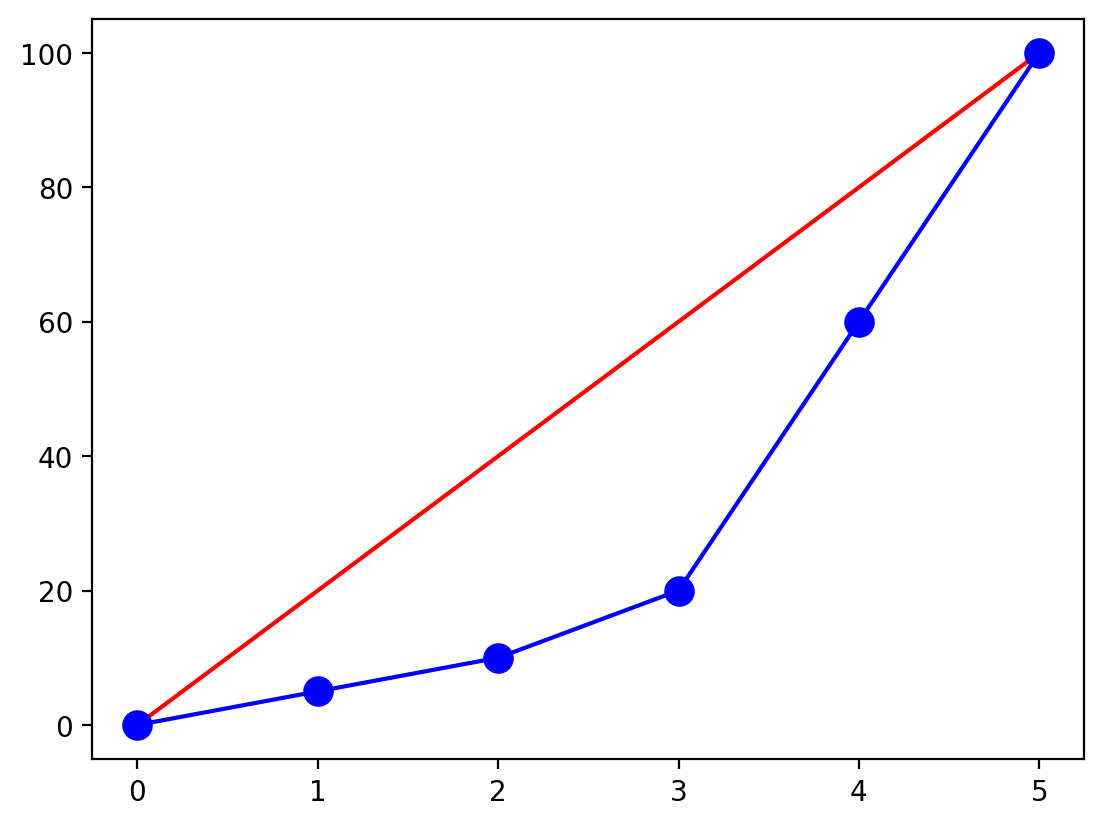
\includegraphics[scale=0.60]{images/exemple_courbe_lorenz_simple.png}
\end{center}

\bigskip

\noindent Encore plus visuellement, une fois la distribution ordonnée, on obtient donc $ 5 \; 5 \; 10 \; 40 \; 40 $.
L'histogramme suivant montre visuellement chaque valeur ajoutée entre les points de la courbe bleue.
Donc, en effectuant la somme des valeurs au fur et à mesure, chaque point de la courbe bleue correspond à $ 5 \; 10 \; 20 \; 60 \; 100 $.

\bigskip

\begin{center}
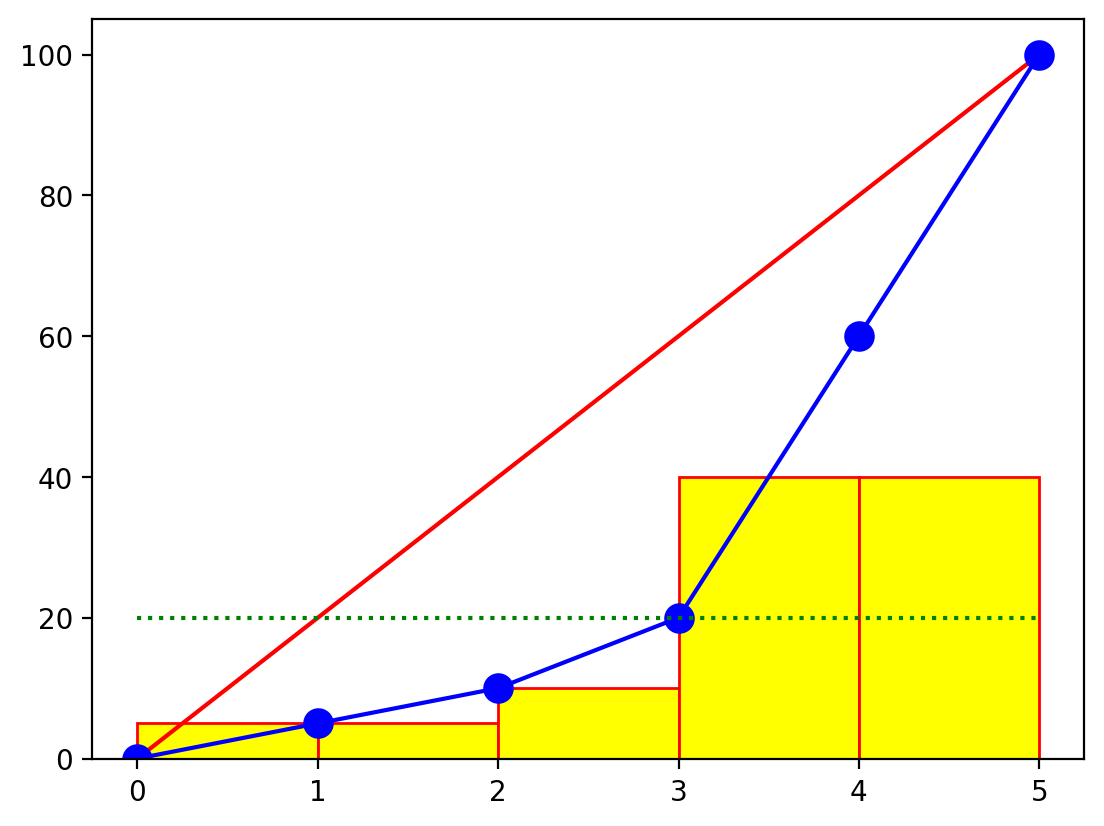
\includegraphics[scale=0.60]{images/exemple_courbe_lorenz-5-5-10-40-40.png}
\end{center}

\bigskip

\noindent Pour rappel, le coefficient de Gini correspond au double de l'aire entre la courbe bleue et la courbe rouge.
Pour bien apprécier visuellement l'écart de cette aire, prenons maintenant deux autres distributions, et comparons l'ensemble des cas :

\begin{itemize}
\item[$\bullet$] $ 0 \; 0 \; 0 \; 10 \; 90 $ (une distribution très inégale) : $ \text{Coeff Gini} = 0,760 $
\item[$\bullet$] $ 5 \; 5 \; 10 \; 40 \; 40 $ (une distribution plutôt inégale) : $ \text{Coeff Gini} = 0,424 $
\item[$\bullet$] $ 10 \; 15 \; 20 \; 25 \; 30 $ (une distribution peu inégale) : $ \text{Coeff Gini} = 0,200 $
\end{itemize}

\bigskip

\noindent Pour bien visualiser ces cas, la moyenne des distributions ($ 20 $) a été tracée en pointillés verts.

\begin{center}
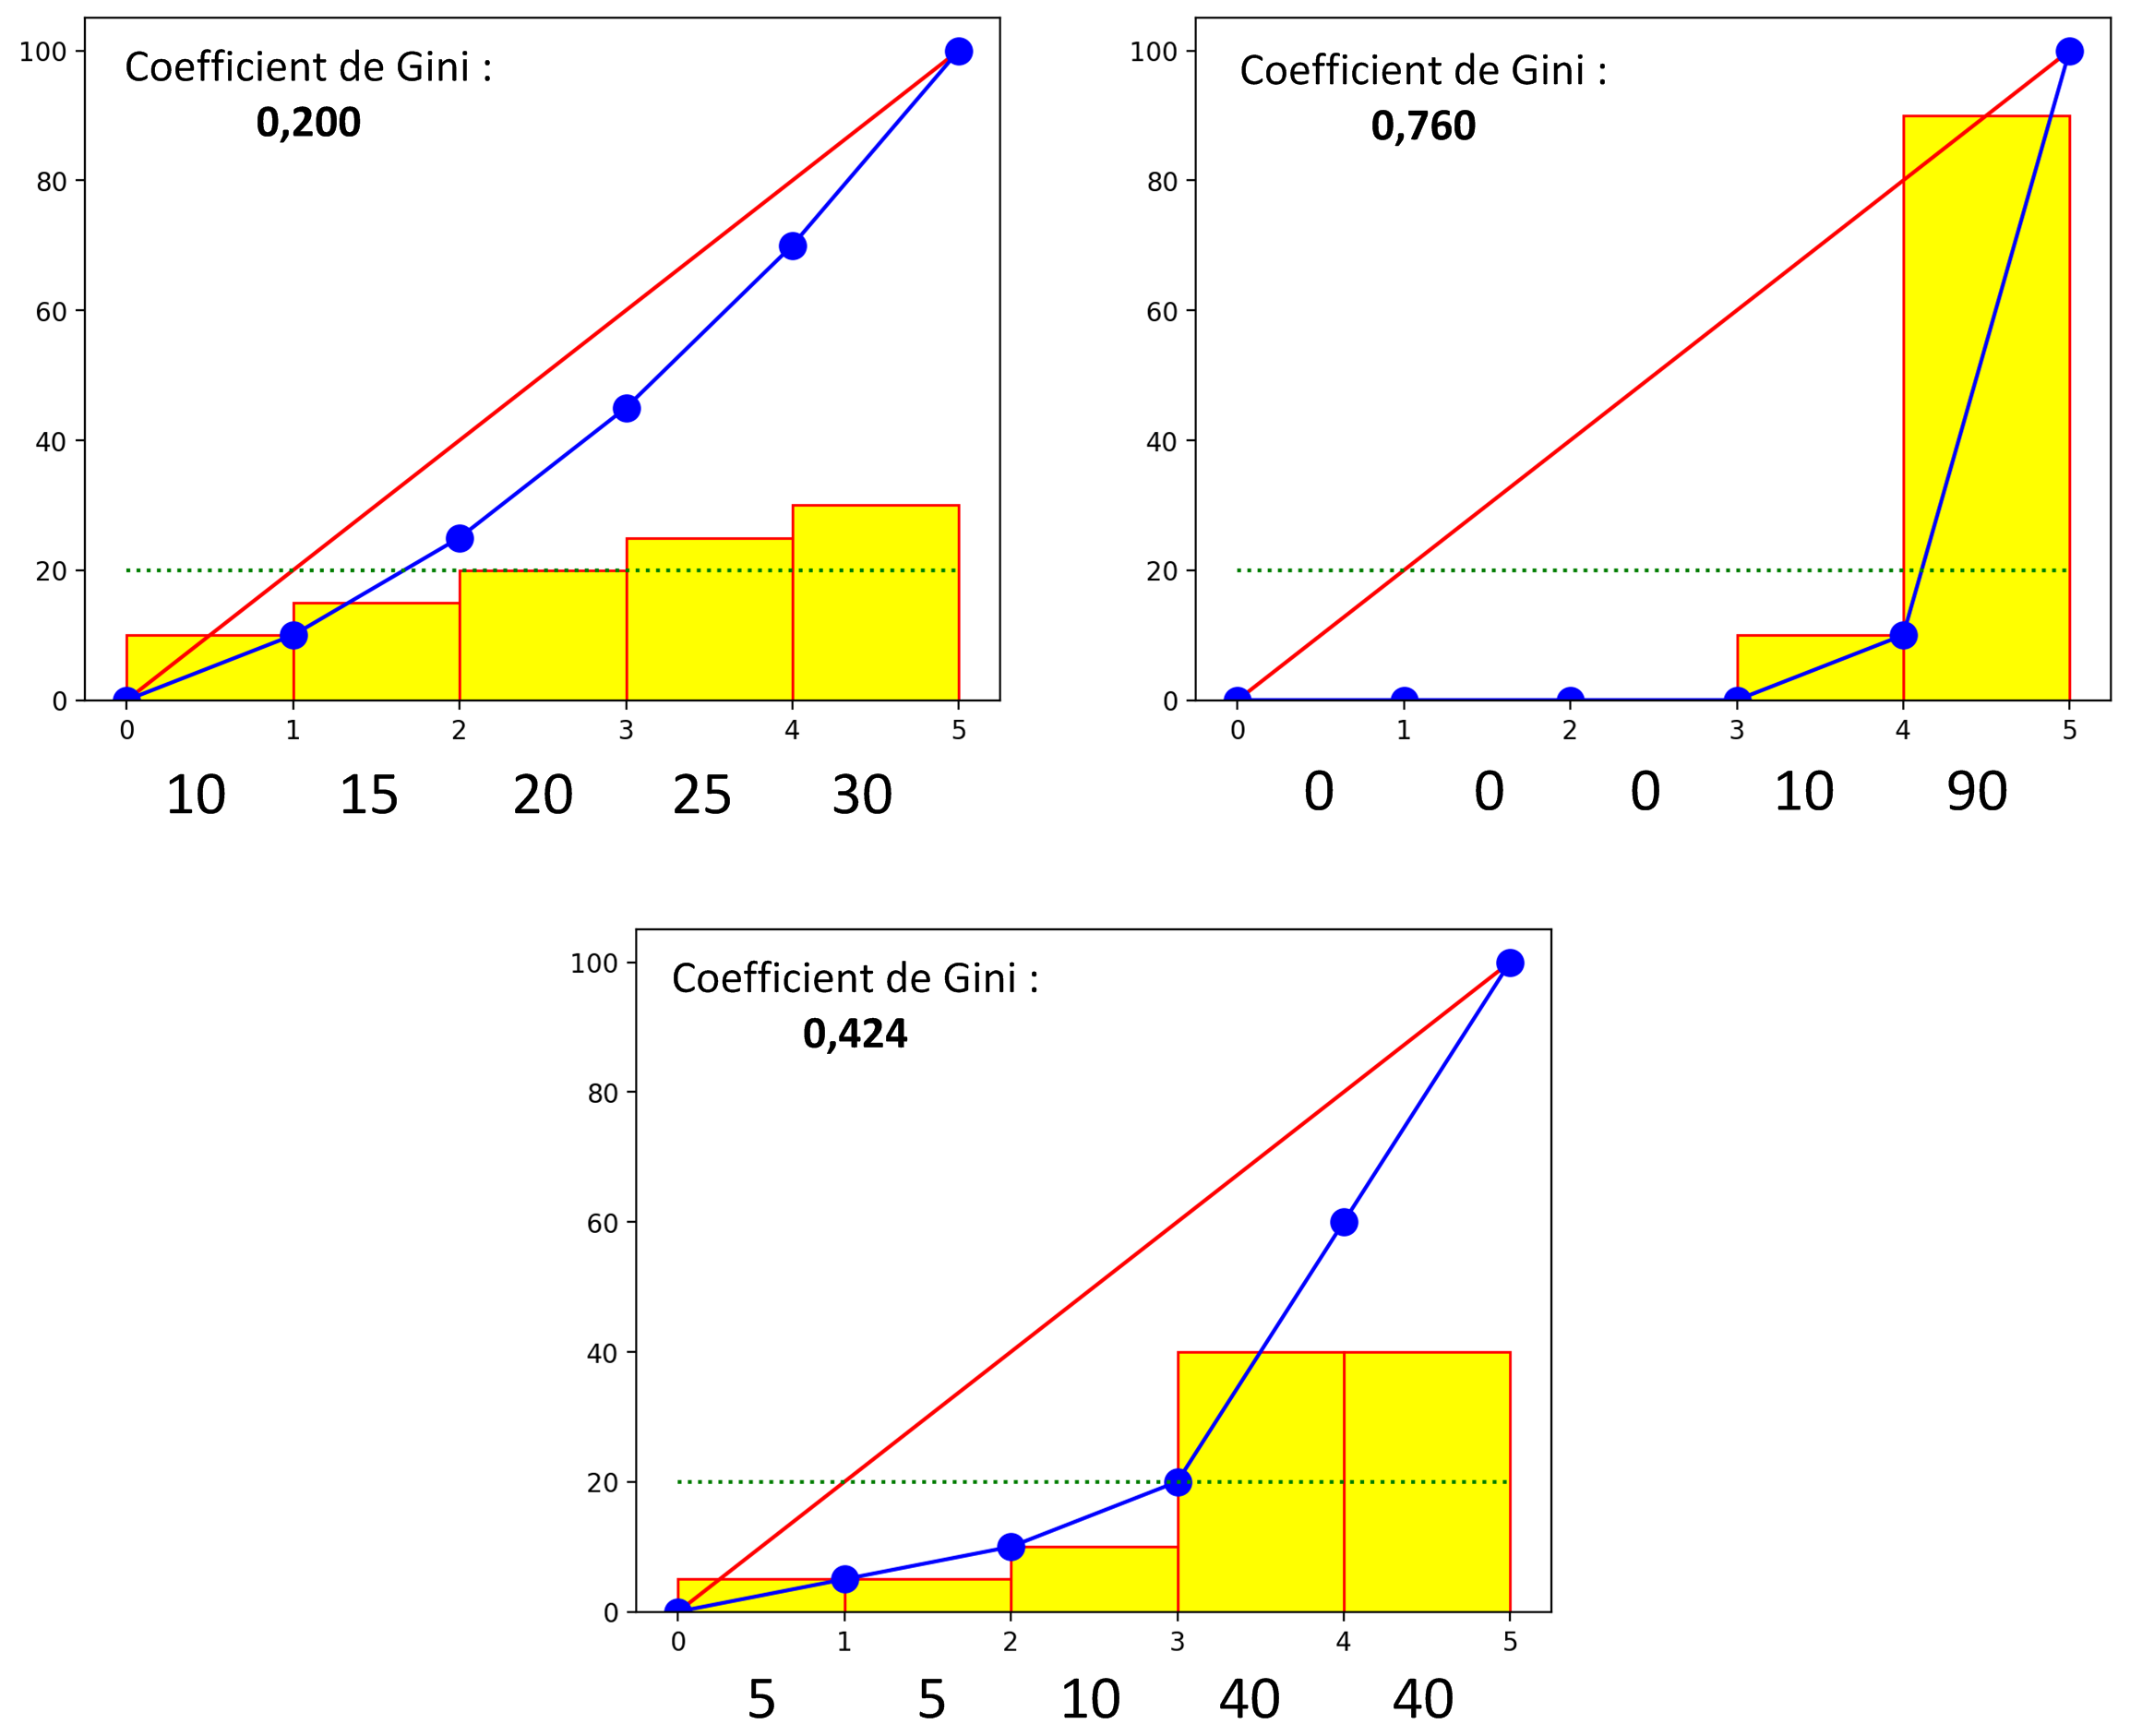
\includegraphics[scale=0.54]{images/exemple_courbes_lorenz.png}
\end{center}

\noindent Comme vous pouvez le constater, le cas peu inégal montre une courbe bleue proche de la courbe rouge, et inversement, le cas très inégal montre une courbe bleue très éloignée de la courbe rouge.
Pour rappel, la moyenne n'est pas un indicateur de dispersion, mais bien un indicateur de tendance centrale ou de position.
Les nombreux indicateurs que vous venez d'implémenter vous permettront donc de mieux interpréter les données dont vous disposerez dans votre carrière, et éventuellement de voir des phénomènes jusque-là peu visibles.

\bigskip

\noindent Reprenons l'implémentation du coefficient de Gini : vous venez de comprendre comment celui-ci est théoriquement construit et interprété.
Mais comment l'implémenter facilement ?

\noindent Deux formules nous intéressent particulièrement, la première est l'équation de Kendal et Stuart.
Dans celle-ci, $ n $ correspond au nombre d'éléments dans la distribution, et $ L_{1} , L_{2} , ... , L_{n} $ correspondent à chaque élément de la distribution.

\begin{center}
\begin{equation*}
G = \frac{ (1 / 2 n^{2}) \, \overset{n}{\underset{i = 1}{\sum}} \overset{n}{\underset{j = 1}{\sum}} \, | L_{i} - L_{j} | }{ (1 / n) \, \overset{n}{\underset{i = 1}{\sum}} \, L_{i}}
\end{equation*}
\end{center}

\noindent En observant cette formule, vous devriez remarquer que la double somme teste littéralement tous les éléments de la distribution deux à deux, ce qui est particulièrement long.
Et qu'il est par la suite nécessaire de diviser le tout par la somme des éléments.

\bigskip

\noindent Si vous implémentez chacune des parties indépendamment, le temps de calcul sera particulièrement long.
Et si vous implémenter toute la formule dans une fonction, vous aurez beaucoup de variables à conserver, et le code risque d'être difficile à comprendre.

\bigskip

\noindent Heureusement, vous devriez remarquer que le diviseur est constitué du nombre d'éléments de la distribution, et de leur somme... ce qui ressemble à la moyenne.
Et effectivement, Mookherjee et Shorrocks ont simplifié cette équation en introduisant la moyenne ($ \mu $) :

% G = \frac{ Moyenne des valeurs absolues des diff\acute{e}rences entre chaque Partie }{ Moyenne de toutes les Parties \times 2}
\begin{center}
\begin{equation*}
G = \frac{1}{2 \mu n^{2}} \, \overset{n}{\underset{i = 1}{\sum}} \overset{n}{\underset{j = 1}{\sum}} \, | L_{i} - L_{j} |
\end{equation*}
\end{center}
% Formule des trapèzes ou Formule des triangles ?
% = AE2 / (W2 * 2)
% AE2 = MOYENNE(ABS(L2-L2); ABS(L2-M2); ..... ; ABS(M2-L2); ABS(M2-M2); ....)
% W2 = MOYENNE(distribution)

\noindent Bien que cette formule semble encore complexe, décomposons-là :

\begin{itemize}
\item[$\bullet$] $ L_{i} - L_{j} $ correspond à la différence entre chaque élément de la distribution.

\item[$\bullet$] $ | L_{i} - L_{j} | $ correspond à la valeur absolue de la différence entre chaque élément de la distribution.

\item[$\bullet$] $ \overset{n}{\underset{i = 1}{\sum}} \overset{n}{\underset{j = 1}{\sum}} \, | L_{i} - L_{j} | $ correspond à la somme des différences absolues des éléments de la distribution. Il s'agit donc de faire une double boucle effectuant la différence entre chaque élément de la distribution, pour ajouter le résultat à une variable initialisée à $ 0 $ juste avant la boucle. La double boucle implique simplement d'itérer comme sur un tableau à deux dimensions ($ | L_{1} - L_{1} | + | L_{1} - L_{2} | + ... + | L_{2} - L_{1} | + | L_{2} - L_{2} | + ... + | L_{n} - L_{n} | $).

\item[$\bullet$] $  2 \mu n^{2} $ correspond simplement à $ 2 $ multiplié par la moyenne de la distribution, multiplié par la quantité d'éléments (le cardinal) au carré.
\end{itemize}


%def CoeffGini(MyDistribution):
%  DiffGini = 0
%  for i in MyDistribution:
%    for j in MyDistribution:
%      DiffGini = DiffGini + abs(i - j)
%  DiffGini = DiffGini / (DistrNbValues ** 2)
%  CoeffGini = DiffGini / (mean(MyDistribution) ** 2)
%  return (CoeffGini)

\bigskip

\noindent Pour conclure, pensez tout de même que le deux formules peuvent être optimisées lors de leur implémentation (on peut calculer la moyenne au fur et à mesure des boucles, ou dans d'autres cas, voire, on peut accumuler la somme des éléments dans une variable).



\end{document}
